%% LyX 2.2.0 created this file.  For more info, see http://www.lyx.org/.
%% Do not edit unless you really know what you are doing.
\documentclass[12pt,a4paper,english,brazil,oldfontcommands]{abntex2}
\renewcommand{\sfdefault}{lmss}
\usepackage[T1]{fontenc}
\usepackage[utf8]{inputenc}
\setcounter{secnumdepth}{3}
\setcounter{tocdepth}{3}
\usepackage{verbatim}
\usepackage{float}
\usepackage{url}
\usepackage{amsmath}
\usepackage{graphicx}
\usepackage{nomencl}
% the following is useful when we have the old nomencl.sty package
\providecommand{\printnomenclature}{\printglossary}
\providecommand{\makenomenclature}{\makeglossary}
\makenomenclature
\OnehalfSpacing

\makeatletter

%%%%%%%%%%%%%%%%%%%%%%%%%%%%%% LyX specific LaTeX commands.
\special{papersize=\the\paperwidth,\the\paperheight}


%%%%%%%%%%%%%%%%%%%%%%%%%%%%%% Textclass specific LaTeX commands.
% adaptação do suporte ao natbib do LyX para uso do abntex2cite
\AtBeginDocument{%                % garante que este código será carregado após
% \usepackage[alf]{abntex2cite} ou
% \usepackage[num]{abntex2cite}
% no preâmbulo latex.
\RequirePackage{abntex2cite}   % previne o não carregamento do abntex2cite,
% mas não define se as citações serão do
% tipo 'alf' ou 'num'.
\renewcommand{\citeauthor}[1]{\citeauthoronline{#1}}
\def\citep{\cite}
\newcommand{\citeyearpar}[1]{(\citeyear{#1})}
\ifx\AbntCitetype\AbntCitetypeALF
\def\citet{\citeonline} % alf
\newcommand{\citealt}[1]{\citeauthoronline{#1}~\citeyear{#1}}
\newcommand{\citealp}[1]{\citeauthoronline{#1},~\citeyear{#1}}
\else
\def\citet{\@ifnextchar[{\citet@with}{\citet@without}} % num
\def\citet@with[#1]#2{\citeauthoronline{#2}~\cite[#1]{#2}}
\def\citet@without#1{\citeauthoronline{#1}~\cite{#1}}
\newcommand{\citealt}[1]{\citeauthoronline{#1}~\citeonline{#1}}
\def\citealp{\citeonline}
\fi
}

%%%%%%%%%%%%%%%%%%%%%%%%%%%%%% User specified LaTeX commands.
\usepackage{indentfirst}
\usepackage{float}
\usepackage{titlesec}
\usepackage{tikz, blindtext}
\usetikzlibrary{shapes.multipart}
\usepackage{calc,soul,fourier}
\usepackage{color, colortbl}
\usepackage{graphicx}
%\usepackage[brazil]{babel}
\usepackage[brazilian,hyperpageref]{backref}
\setlength{\parindent}{48pt}
\usepackage[alf]{abntex2cite}
%\usepackage{lmodern}
\usepackage[unicode=true]{hyperref}
\hypersetup{%
pdfborder = {0 0 0},
colorlinks ,
citecolor=blue,
filecolor=blue,
linkcolor=blue,
urlcolor=blue
}


%================================================================================
%======================================
%estilo do section, subsection e subsubsection
%======================================
 
\titleformat{\section}
{\normalfont\fontsize{16pt}{18pt}\selectfont\bfseries}{\thesection}{1em}{}
\titleformat{\subsection}
{\normalfont\fontsize{14pt}{16pt}\selectfont\bfseries}{\thesubsection}{1em}{}
\titleformat{\subsubsection}
{\normalfont\fontsize{12pt}{14pt}\selectfont\bfseries}{\thesubsubsection}{1em}{}


%================================================================================
%======================================
%Pacotesdecitações
%======================================
\renewcommand*{\backref}[1]{}
\renewcommand*{\backrefalt}[4]{
\ifcase #1 (No citado.)
\or (Citado na página~#2.)
\else (Citado nas páginas #2.)
\fi%
}
\renewcommand*{\backrefsep}{, }
\renewcommand*{\backreftwosep}{e~}
\renewcommand*{\backreflastsep}{e~}
%================================================================================
% Configuração dos Estilo dos Capítulo
%================================================================================

\makechapterstyle{box}{

\renewcommand{\chapterheadstart}{}
% Secao secundaria (Section) Caixa baixa, Negrito
\renewcommand*{\cftsectionfont}{\bfseries}
% Secao terciaria (Subsection) Caixa baixa, Negrito, italico
\renewcommand*{\cftsubsectionfont}{\itshape\bfseries}
% Secao quaternaria (Subsubsection) Caixa baixa, italico
\renewcommand*{\cftsubsubsectionfont}{\itshape}
% Secao quinquenária (Subsubsubsection) Caixa baixa
\renewcommand*{\cftparagraphfont}{\normalsize}

% tamanhos de fontes de chapter e part
\ifthenelse{\equal{\ABNTEXisarticle}{true}}{%
\setlength\beforechapskip{\baselineskip}
\renewcommand{\chaptitlefont}{\ABNTEXsectionfont\ABNTEXsectionfontsize}
}{%else
\setlength{\beforechapskip}{0pt}
\renewcommand{\ABNTEXchapterfontsize}{\LARGE}
%\renewcommand{\ABNTEXchapterfont}{\sffamily\bfseries}
%alteração da fonte dos capítulos, seções e subseções
\renewcommand{\chaptitlefont}{\ABNTEXchapterfont\bfseries\ABNTEXchapterfontsize}
}
%\renewcommand{\chapter}{\chaptertitlename\ \thechapter}{0pt}{\Large\uppercase}
\renewcommand{\chapnumfont}{\chaptitlefont}
\renewcommand{\parttitlefont}{\ABNTEXpartfont\ABNTEXpartfontsize}
\renewcommand{\partnumfont}{\ABNTEXpartfont\ABNTEXpartfontsize}
\renewcommand{\partnamefont}{\ABNTEXpartfont\ABNTEXpartfontsize}

\renewcommand*{\printchaptername}{}
\renewcommand*{\chapnumfont}{\normalfont\sffamily\huge\bfseries}
\renewcommand*{\printchapternum}{
\hrulefill{\renewcommand{\arraystretch}{1.5}
\begin{tabular}{|c|}
\rowcolor{black}\color{white}\normalsize\ABNTEXchapterfont\MakeTextUppercase{\chaptername}\\
\vspace{-1.5ex}\\
\resizebox{!}{1.1cm}{\ABNTEXchapterfont\thechapter}
\\[2.5ex]
\hline
\end{tabular}
}
}

\renewcommand*{\chaptitlefont}{\normalfont\sffamily\Huge\bfseries}
\renewcommand*{\printchaptertitle}[1]{
\flushright\chaptitlefont##1
\vskip -0.6ex\hfill\rule{.8\textwidth}{0.5pt} \\
\vskip -2.8ex\hfill\rule{.8\textwidth}{2pt}\\
\vskip 1.5ex
}

}

\chapterstyle{box}

%=================================
%Configurações do estilo da pagina
%==================================

%\makepagestyle{ruled}
%\makeoddfoot{ruled}{}{}{}
%\makeevenfoot{ruled}{}{}{}
%\makeheadrule{ruled}{\textwidth}{\normalrulethickness}
%\makeevenhead{ruled}{\thepage}{}{\small\itshape\leftmark}
%\makeoddhead{ruled}{\small\itshape\rightmark}{}{\thepage}
%\makeatletter % because of \@chapapp
%\makepsmarks  {ruled}{
%\nouppercaseheads
%\createmark	{chapter} 	{both} {shownumber}{\@chapapp\ }{. \ }
%\createmark	{section} 	{right} {shownumber}{}		  {. \ }
%\createplainmark {toc}		{both}{\contentsname}
%\createplainmark {bib}		{both}{\bibname}
%}
%\makeatother
%\pagestyle{ruled}

%================================================================================
% Configuração das legendas nas figuras e tabelas
%================================================================================

\newcommand{\fautor}{\legend{Fonte: Elaborada pelo autor.}}
\newcommand{\fadaptada}[2][]{\legend{Fonte: Adaptada de \citeonline[#1]{#2}.}}
\newcommand{\fdireta}[2][]{\legend{Fonte: \citeonline[#1]{#2}.}}
\newcommand{\fdadospesquisa}{\legend{Fonte: Dados da pesquisa.}}

%\usepackage{lmodern}
\newcommand{\blankpage}{
\newpage
\thispagestyle{empty}
\mbox{}
\newpage
}
\setcounter{secnumdepth}{4}

\makeatother

\usepackage{babel}
\usepackage{listings}
\addto\captionsbrazil{\renewcommand{\lstlistingname}{\inputencoding{latin9}Listagem}}
\addto\captionsenglish{\renewcommand{\lstlistingname}{\inputencoding{latin9}Listing}}
\renewcommand{\lstlistingname}{\inputencoding{latin9}Listagem}

\begin{document}
%Configurações do estilo da pagina %==================================
\makepagestyle{ruled} 
\makeoddfoot{ruled}{}{}{}   
\makeevenfoot{ruled}{}{}{}   
\makeheadrule{ruled}{\textwidth}{\normalrulethickness}   
\makeevenhead{ruled}{\thepage}{}{\small\itshape\leftmark}   
\makeoddhead{ruled}{\small\itshape\rightmark}{}{\thepage} 
\makeatletter % because of \@chapapp      
\makepsmarks  {ruled}{  
\nouppercaseheads 
\createmark	{chapter} 	{both} {shownumber}{\@chapapp\ }{. \ } 
\createmark	{section} 	{right} {shownumber}{}		  {. \ } 
\createplainmark {toc}		{both}{\contentsname} 
\createplainmark {bib}		{both}{\bibname}}
\makeatother 
\pagestyle{ruled}

\cleardoublepage{}

\cleardoublepage{}

\cleardoublepage{}

\cleardoublepage{}

\cleardoublepage{}

\cleardoublepage{}

\newpage{}

\clearpage{}

\renewcommand{\nomname}{Lista De Abreviaturas e Siglas}

\clearpage{}

\chapter{Introdução}

Os Sistemas de Apoio à Decisão (SAD \nomenclature{SAD}{Sistemas de Apoio à Decisão})
organizam e processam os dados e informações para gerar resultados
de valor que auxiliem o processo de decisão em um domínio especifico,
ditos sistemas integram conhecimento desenvolvido pelos especialistas
do domínio que fica implícito nos dados, informações e processos,
dito conhecimento não é familiar para os desenvolvedores de software,
o que leva a usar diversas técnicas de levantamento de requerimentos
que envolvem o aprendizado de tópicos do domínio dos especialistas
por parte dos desenvolvedores, este processo exige um esforço adicional
por parte dos desenvolvedores do sistema e traz limitações no tempo
e custo de desenvolvimento, devido a que o conhecimento precisa ser
explicado por parte dos especialistas do domínio aos desenvolvedores
de software, para que eles consigam entender o conhecimento e assim
implementar o sistema software corretamente.

Adicionalmente, os especialistas do domínio pelo geral não tem o conhecimento
de desenvolvimento de sistemas software para realizar dito processo
por eles mesmos; alem disso os dois domínios, tanto dos especialistas
do domínio como do desenvolvimento de software são tão amplos que
precisam perfis particulares para realizar os processos corretamente,
devido ao anterior foi identificado o problema da inexistência de
uma representação de conhecimento para definir SADs, que tenha um
formato computável, entendível e acessível pelos especialistas do
domínio e desenvolvedores de software.

Como exemplo do anterior problema, podermos expor o caso dos especialistas
em sustentabilidade da Embrapa Meio Ambiente, que desenvolveram o
projeto SustenAgro (capitulo \ref{chap:Sustainability_Assessment}),
onde foi desenvolvido um método de avaliação de sustentabilidade no
sistema produtivo de cana-de-açúcar, os especialistas precisavam implementar
um SAD para disponibilizar o uso do método à comunidade interessada
em realizar avaliações de sustentabilidade em cana-de-açúcar, , no
caso deles foi identificado que tinham o conhecimento do domínio avaliação
de sustentabilidade da cana-de-açúcar, mas não tinham o método e ferramenta
software para definir dito conhecimento de maneira computável em um
SAD, pelo que dito problema e caso de uso foram abordados na presente
pesquisa como projeto piloto.

\section{Motivação}

A pesquisa em representação e organização de conhecimento tem alto
impacto devido a fornece métodos e ferramentas para gerenciar o conhecimento
em diversos domínios, especificamente no desenvolvimentos dos SADs,
pode fornecer meios de integração de conhecimento que aumentam as
funcionalidades e a eficiência desses sistemas em comparação com os
métodos tradicionais de desenvolvimento.

Sobre o caso especifico do projeto SustenAgro, existem varias motivações
para desenvolver novos meios de definição de SAD, entre eles está
principalmente o fornecimento de um método e ferramenta para que os
especialistas do domínio definiam o conhecimento nos SADs, permitindo
a participação deles como descritores de conhecimento especifico,
também temos que a avaliação da sustentabilidade da cultura de cana-de-açúcar
está em continua mudança \citep{oliveira:2013}, pelo que existe a
necessidade de fornecer meios computáveis de representação desse conhecimento
que adaptem-se às mudanças do domínio e que facilite a comunicação
entre os especialistas do domínio e os desenvolvedores de software.

Além disso, permitira definir SADs com menos intervenção por parte
dos não especialistas do domínio, fazendo que a definição do conhecimento
fique em termos dos especialistas e gerenciadas por eles mesmos, fornecendo
a possibilidade de que descrevam características particulares que
requerem profundo conhecimento do domínio, finalmente fornecera aos
desenvolvedores tempo adicional para dedicar-se aos assuntos próprios
da computação, e assim agilizar o processo de desenvolvimento de SADs.

Na representação de conhecimento existem vários tipos de sistemas
de organização de conhecimento (\nomenclature{KOS}{Knowledge Organization System}
pelas siglas em inglês), um dos sistemas mais completos são as ontologias
que permitem definir, classificar, relacionar e inferir conhecimento,
e como deseja-se um meio que suporte vários aspectos do conhecimento,
se definiu usar este tipo de \foreignlanguage{english}{KOS} no processo
de modelagem, fornecendo um caso real de aprendizagem e implementação
de ontologias.

A Embrapa Meio Ambiente também tem outros SAD que podem ser avaliados
e modelados com a finalidade de desenvolver um método e ferramenta
geral de definição de SADs.

\section{Objetivo}

Desenvolver um método e ferramenta web baseados em ontologias que
permita representar o conhecimento dos especialistas do domínio para
suportar definição de SADs, e provar o funcionamento por meio da definição
do SAD SustenAgro, que tem como finalidade suportar a avaliação da
sustentabilidade nos sistemas produtivos de cana-de-açúcar no centro-sul
do Brasil 

Para atingir o objetivo proposto, foi necessário atingir os seguintes
objetivos específicos: 

\subsection*{Objetivos específicos}
\begin{itemize}
\item Desenvolver um método de definição de SAD por parte dos especialistas.
\item Definir uma arquitetura e ferramenta para definir SADs baseados em
conhecimento de domínios específicos.
\item Desenvolver uma ontologia sobre avaliação da sustentabilidade nos
sistemas produtivos de cana-de-açúcar do centro sul do Brasil, como
base conceitual e tecnológica do sistema SustenAgro.
\item Desenvolver uma ontologia sobre controles visuais para suportar a
geração da interface gráfica do SAD SustenAgro.
\item Desenvolver uma DSL que gerencie as ontologias e que flexibilize a
definição da interface de usuário por parte dos administradores do
sistema.
\item Demonstrar que o método e ferramenta de definição de SADs por parte
dos especialistas, permite a geração de sistemas funcionais.
\end{itemize}

\section{Resultados Principais}

Os principais resultados desta pesquisa e projeto de mestrado são:
\begin{itemize}
\item Método e ferramenta para definir SADs por parte dos especialistas
do domínio.
\item Ontologia sobre avaliação de sustentabilidade em cana-de-açúcar, representando
os principais conceitos desse domínio: indicadores, os índices e o
método de avaliação; permitindo assim suportar o desenvolvimento das
outras tecnologias do presente projeto.
\item Ontologia sobre interfaces gráficas que permite representar os tipos
de dados e \foreignlanguage{english}{widgets} necessários para a geração
dos Sistemas de Apoio na Decisão.
\item DSL: linguagem de domínio especifico que permite gerenciar ontologias
para definir sistemas de apoio à decisão.
\item Protótipo do Decisioner: Sistema gerador de SADs, que suporta a integração
de ontologias e DSL em ambientes web.
\item SustenAgro: Sistema de Apoio a Decisão para avaliar a sustentabilidade
em cana-de-açúcar, implementado o método SustenAgro e tecnologias
da web semântica.
\item Artigo ``\foreignlanguage{english}{Sustainability assessment of sugarcane
production systems: SustenAgro Method}'' submetido no periódico acadêmico
``\foreignlanguage{english}{Energy for sustainable Development}''
ISSN: 0973-0826 submetido na data 23 de dezembro do 2016. 
\end{itemize}

\section{Organização}

Este trabalho de dissertação está estruturado da seguinte forma: 

Capítulo 2: Apresenta o SAD SustenAgro e os trabalhos relacionados
sobre geração de Sistemas de Apoio à Decisão e os Sistemas de Avaliação
da Sustentabilidade para representar o estado da arte da presente
pesquisa.

Capítulo 3: Apresenta a fundamentação teórica sobre Ontologias e DSL
com a finalidade de descrever as principais tecnologias e a teoria
necessária para desenvolver o presente trabalho.

Capítulo 4: Apresenta o protótipo do sistema Decisioner que permite
suportar a geração de Sistemas de Apoio à Decisão. 

Capítulo 5: Apresenta o SAD SustenAgro, desenvolvido na presente pesquisa
e que se serviu como primeiro caso de uso do sistema Decisioner, para
definir a arquitetura dele e demostra a funcionalidade do sistema
desenvolvido.

Capítulo 6: Apresenta a avaliação realizada pelos especialistas.

Capítulo 7: Apresenta as conclusões do presente trabalho, uma discussão
e possíveis trabalhos futuros.

Finalmente são apresentados os anexos que descrevem conceitos específicos
do trabalho.


\chapter{Web semântica}

\input{\string"chapters/Semantic Web.tex\string"}

\chapter{SAD}

A construção de sistemas que sejam capazes de fornecer suporte ao
gestor em um processo de tomada de decisões tem sido um desafio ao
longo dos anos. A continuação será explicado a definição e arquitetura
de SAD, o SAD SustenAgro e os trabalhos relacionados.

\section{Definição de SAD}

Os Sistemas de Apoio à Decisão (SAD) são uma área de conhecimento
ampla e em continua evolução. A definição de SAD deriva da definição
de sistema, pois eles contêm um conjunto de partes organizadas para
um proposito comum, existem múltiplas definições do termo SAD, a continuação
serão apresentadas algumas definições que permitem explicar o proposito
deste tipo de sistemas.

\citet{Tweedale2016} define os SADs como sistemas software que visam
melhorar a tomada de decisão individual ou grupal, combinando o conhecimento
do(s) tomador(es) de decisão com dados relevantes de fontes confiáveis,
nos quais são aplicados métodos e modelos matemáticos para suportar
a análise, comparação e escolha de alternativas no processo de decisão.

\citet{heinzle2010semantica} define que os SADs apoiam o entendimento
de processos complexos, auxiliam na comparação dos fenômenos envolvidos
e suportam a análise e escolha de alternativas no processo de decisão.
Este entendimento do domínio surge da combinação das habilidades e
metodologias dos especialistas (humanos) à capacidade dos computadores
de acessar dados, estruturá-los em modelos, interpretar, formular
e avaliar alternativas e cenários distintos.

O conhecimento dos especialistas do domínio está implícito nos SADs.
\citet{Evans:2003:DDT:861502} explica que existe uma necessidade
de modelar o conhecimento chave de um domínio em um modelo, para permitir
a comunicação e colaboração entre especialistas de domínio e os desenvolvedores,
pelo qual o modelo de conhecimento dos especialistas será objeto da
pesquisa. O processo de modelagem pode ser lento e custoso, já que
os dois grupos de profissionais têm \foreignlanguage{english}{\emph{Backgrounds}}
diferentes, que dificultaram o processo de desenvolvimento e testes
de um SAD.

Os especialistas de domínio e os desenvolvedores, pelo geral são de
organizações diferentes, o que dificulta ainda mais o processo, pelo
qual foram pesquisados modelos que facilitem o entendimento entre
os dois tipos de profissionais e desenvolvida uma pesquisa ao redor
deste tópico.

A continuação será apresentada a arquitetura dos SAD e a importância
dos modelos de conhecimento existentes dentro um SAD. 

\section{Arquitetura para Sistemas de Apoio à Decisão}

A arquitetura de um software define a organização dele em termos de
componentes, de interconexões, e das interações com sistemas externos
\citep{de1997software}. A arquitetura fornece as informações de como
os componentes dela se relacionam, explicando a parte externa das
ligações entre seus elementos, sendo que as implementações internas
não são consideradas parte da arquitetura \citep{sei2006architecture}.

Estas partes são descritas por meio da arquitetura representada na
figura \ref{fig:Componentes-SAD}, representando o processo realizado
pelos SADs, no qual recebem uma entrada, fazem o processamento dela
e retorna resultados que são analisadas pelo tomador(es) de decisão
a través da tecnologia computacional \citep{Tweedale2016}. 

\begin{figure}[H]
\noindent \begin{centering}
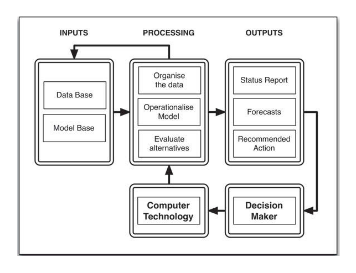
\includegraphics[width=0.8\columnwidth]{figures/DSS}
\par\end{centering}
\caption{Componentes de um SAD.\label{fig:Componentes-SAD} }

\fadaptada{Tweedale2016}
\end{figure}

A Figura \ref{fig:Componentes-SAD} mostra os componentes de um SAD,
que são: 
\begin{description}
\item [{I\foreignlanguage{english}{nputs}}] corresponde às entradas do
sistema, composta dos dados que serão processados e dos modelos de
conhecimento dos especialistas. Os dados estão armazenados em bancos
de dados e os modelos pelo geral estão implícitos no SAD ou podem
estar em uma base de conhecimento. Esses dois componentes devem ser
o mais precisos e completos possíveis para garantir respostas confiáveis
do sistema.
\selectlanguage{english}%
\item [{Processing}] \foreignlanguage{brazil}{está composto pelos modelos
e métodos de organização e processamento dos dados, que tem restrições
para avaliar as alternativas de resposta. Os métodos podem ser de
tipo matemáticos, que processam os dados e geram os resultados do
sistema.}
\item [{Outputs}] \foreignlanguage{brazil}{são os resultados do processamento
dos inputs e permitem comparar as alternativas de decisão. As saídas
comuns são relatórios, previsões e recomendações, que são apresentados
por meio de uma interface de usuário para facilitar o entendimento
e interação por parte dos usuários.}
\end{description}
Durante a evolução dos SAD, várias melhorias aconteceram, entre elas
o desenvolvimento da Web permitiu integrar novas técnicas no processamento
dos dados, tecnologias na representação visual de resultados e no
uso colaborativo por parte dos usuários \citep{Shim2002}. Também
existe a tendência da integração com métodos de inteligência artificial,
para estender a aplicabilidade dos SAD a problemas complexos. 

Uma variação dos SADs integra bases de conhecimento que suportam inferência,
permitindo o desenvolvimento de \foreignlanguage{english}{Expert Systems}
e \foreignlanguage{english}{Knowledge Based Systems.} Esses sistemas
são classificados como \foreignlanguage{english}{Rule Based Systems}
\citep{Tweedale2016}, os quais estabelecem o escopo desta pesquisa. 

Um tipo de SAD que usa bases de conhecimento, são os que usam ontologias
para representar o conhecimento dos especialistas, permitindo definir,
classificar, relacionar e inferir conhecimento. 

A continuação será apresentado o SAD SustenAgro baseado em conhecimento,
que suporta a avaliação da sustentabilidade em cana-de-açúcar a través
do uso de ontologias.

\section{SAD SustenAgro\label{sec:SAD-SustenAgro}}

Um domínio de conhecimento caracterizado pela sua complexidade são
os sistemas produtivos agrícolas. Eles envolvem fenômenos de natureza
diversa \citep{simon1991architecture}, integrando aspectos ambientais,
sociais e econômicos.

Particularmente, o setor produtivo produtivo da cana-de-açúcar é extremamente
importante para a economia do estado de São Paulo e do Brasil, devido
ao fato de ser uma das principais culturas produzidas no país \citep{Storquato2015}.
Atualmente a cana-de-açúcar é a mais importante fonte de energia renovável
no Brasil \citep{seabra2011life}, permitindo a produção de etanol
e energia eléctrica, além de ter mais de 20 subprodutos, entre eles
açúcar, etanol, bioeletricidade, bioplásticos e Hidrocarbonetos \footnote{\url{http://sugarcane.org/sugarcane-products}}. 

A produção da cana-de-açúcar e dos subprodutos dela, influem em aspectos
ambientais consumindo recursos naturais, em aspectos sociais envolvendo
pessoas na produção e em aspectos econômicos na comercialização. Esses
aspectos fazem complexo manter a produtividade atualmente e no futuro.
Por essas razões, a Embrapa Meio Ambiente escolheu especificamente
o sistema produtivo da cultura de cana-de-açúcar na região centro-sul
do Brasil, como sistema piloto para desenvolver métodos e software
de avaliação da sustentabilidade (apêndice \ref{chap:Sustainability_Assessment}).

Dada a complexidade da análise da sustentabilidade em sistemas de
produção agrícola, os pesquisadores da Embrapa Meio Ambiente trabalharam
na definição de métodos que permitissem avaliar a sustentabilidade
de maneira integral \citep{Singh2012281}. Por essa razão, desenvolveram
um método que aborda a avaliação em termos de indicadores, simplificando
a complexidade deste sistema agrícola. Cada indicador mede um determinado
aspecto crítico no sistema produtivo, para determinar o quão sustentável
ele é. A partir da análise de cada indicador, é possível gerar recomendações
de medidas corretivas para as unidades produtivas ou para o embasamento
de políticas públicas que incentivem a sustentabilidade. A definição
conceitual do processo de avaliação está detalhada no apêndice \ref{chap:Sustainability_Assessment}. 

A partir do método de avaliação SustenAgro, foi desenvolvida uma ferramenta
de avaliação da sustentabilidade intitulada SAD SustenAgro que implementa
o método SustenAgro por meio de um sistema de apoio a decisão e que
consegue adaptar-se às mudanças do domínio.

O SAD SustenAgro suporta a avaliação da sustentabilidade em cana-de-açúcar
no centro-sul do Brasil. A figura \ref{fig:SustenAgro-arquitetura-inicial}
apresenta a arquitetura inicial do SAD SustenAgro, a qual corresponde
a um sistema de informação tradicional, que requer a intervenção de
desenvolvedores de software, para definir ou atualizar o conhecimento
dos especialistas implícito no SAD.

\begin{figure}[h]
\begin{centering}
\includegraphics[width=0.6\columnwidth]{\string"figures/SustenAgro Initial Architecture\string".eps}
\par\end{centering}
\caption{SustenAgro arquitetura inicial.\label{fig:SustenAgro-arquitetura-inicial}}
\end{figure}

Os especialistas em sustentabilidade definiram o SAD Sustenagro com
as seguintes características:
\begin{itemize}
\item Sistema web com banco de dados para armazenar e recuperar as informações
do sistema.
\item Integração e implementação do método SustenAgro de avaliação de sustentabilidade,
descrito no apêndice \ref{chap:Sustainability_Assessment} 
\item Flexibilidade para adaptar o método SustenAgro a outras culturas.
\item Integração com sistemas de georreferenciamento.
\item Desenvolvimento de \foreignlanguage{english}{widgets} especificas
\footnote{\selectlanguage{english}%
Widgets\foreignlanguage{brazil}{ refere-se à componentes visuais dos
sistemas web }\selectlanguage{brazil}%
} para mostrar resultados obtidos: \foreignlanguage{english}{Sustainability
Matrix }e \foreignlanguage{english}{Sustainability Semaphore,} explicadas
no capítulo \foreignlanguage{english}{\ref{chap:SustenAgro}}
\item Geração de relatórios e de recomendações de sustentabilidade.
\end{itemize}
Um dos problemas identificados foi que os especialistas não tinham
uma definição clara do SAD SustenAgro. Pelo que foi necessário realizar
um levantamento de requisitos, descrito no capítulo \ref{chap:SustenAgro},
para definir os requisitos funcionais (essenciais) e não funcionais
(desejáveis). Além disso, foi necessário reestruturar o desenvolvimento
do SAD SustenAgro para que fizesse parte do processo de pesquisa.

O SAD SustenAgro faz parte de um conjunto de ferramentas de avaliação
definidas pela Embrapa Meio Ambiente. A partir do analise das ferramentas
similares ao SAD SustenAgro, foi evidenciada a necessidade de fornecer
métodos e ferramentas computacionais que organizem a informação. Para
apoiar aos especialistas a tomar decisões baseadas em conhecimento,
permitindo simplificar a resolução de problemas que de outra maneira
não seriam triviais. 

Exatamente foi identificado que ditos sistemas tinham em comum um
método de avaliação que processava de maneira matemática um conjunto
de dados e gerava relatórios com resultados da avaliação, gráficos
e recomendações. As ferramentas analisadas foram:
\begin{enumerate}
\item Sistema Innova-Tec: avaliação do impacto da inovação tecnológica\footnote{\url{http://www.cnpma.embrapa.br/forms/inova_tec.php3}}.
\item Sistema Nano-Tec: avaliação do impacto das nanotecnologias\footnote{\url{https://www.embrapa.br/en/busca-de-publicacoes/-/publicacao/951543/metodologia-para-avaliacao-de-impactos-das-nanotecnologias-metodo-e-software-impactos-nanotec} }.
\item Sistema GMP-RAM v.1.1: avaliação de Risco de Plantas Geneticamente
Modificadas (GMP \nomenclature{GMP}{Genetically Modified Plants})\footnote{\url{http://www.cnpma.embrapa.br/forms/gmp_ram.php3}}
\item Software para avaliação de segurança e impactos de plantas geneticamente
modificadas\footnote{\url{http://www.cnpma.embrapa.br/nova/mostra2.php3?id=857}}
\item Sistema Atlantis: Sistema para levantamento e sistematização da informação
técnica em temas de pesquisa, tecnologias e inovação. \footnote{\url{https://www.embrapa.br/en/busca-de-produtos-processos-e-servicos/-/produto-servico/2102/atlantis---atlantis}}
\end{enumerate}
Uma característica importante em ditos sistemas foi a existência de
conceitos de domínio especifico na organização dos dados de entrada
dos SAD e no método de avaliação. Esta característica permite identificar
que cada um dos sistemas requiriu um processo de modelagem dos conceitos
do domínio por parte dos desenvolvedores. 

Principalmente identificou-se que a implementação desse conhecimento
gerava dificuldades de compreensão entre os especialistas do domínio
e os desenvolvedores de software por serem de áreas diferentes. \citet{Evans:2003:DDT:861502},
propõe que este conhecimento deve ser representado em um modelo independente.

Baseando-se no anterior, afirmou-se a hipótese de usar um modelo para
representar dito conhecimento. E baseando-se no problema de pesquisa,
as ontologias foram selecionadas como o modelo mais completo para
representar o conhecimento do domínio dos especialistas na definição
de SAD, e evitar que o conhecimento ficara implícito como aconteceu
nos SAD listados.

O uso de uma ontologia permitirá representar e estruturar o conhecimento
de avaliação da sustentabilidade em agricultura, a través da definição
e atualização de conceitos por parte dos especialistas, permitindo
que eles mesmos descrevam o domínio sem precisar dos desenvolvedores.
Os especialistas do domínio tem familiaridade com os termos da ontologia
e poderão especificar grande parte do conhecimento envolvido no SAD.
Idealmente, essa definição deve ser detalhada o suficiente para que
os desenvolvedores possam desenvolver a parte computacional do SAD
sem necessidade de \foreignlanguage{english}{feedback} dos especialistas.

Esta representação de conhecimento pode ser mais exata da realidade
do que outros modelos, devido a que está em um formato voltado a descrição
de conhecimento, sobre o qual é possível fazer inferências e assim
gerar informações para suportar a decisão. A partir dessa definição
computável será gerado o SAD SustenAgro. 

Devido a este contexto, o SAD SustenAgro foi escolhido como projeto
piloto para desenvolver a presente pesquisa, porque permite o desenvolvimento
de um SAD baseado em conhecimento e que permite explorar alternativas
na definição e geração dos SAD.

\section{Trabalhos relacionados}

Com a finalidade de relacionar pesquisas sobre o tema que forneçam
ideias e exemplos para abordar o problema, realizou-se uma consulta
na literatura por SADs que usassem ontologias do domínio dos especialistas,
e SADs semelhantes ao SustenAgro. Foi feita uma pesquisa bibliográfica
utilizando fontes de informação acadêmica.

Sobre o uso de ontologias em domínios similares ao SustenAgro:

O vocabulário\emph{ }\foreignlanguage{english}{\emph{Agricultural
Vocabulary (AGROVOC\nomenclature{AGROVOC}{Agricultural vocabulary})}}
\footnote{Definição do Agrovoc\url{http://aims.fao.org/agrovoc}}
que é um \foreignlanguage{english}{\emph{thesaurus}} (sistema de referência
de termos) fornece termos padronizados sobre alimentação, nutrição,
agricultura, pesca, floresta e meio ambiente criados de maneira colaborativa
e coordenados pela \foreignlanguage{english}{\emph{Food and Agricultural
Organization}}\emph{ }\footnote{\emph{Site da FAO \url{http://www.fao.org/home/en/}}}\emph{(FAO}). 

Esses termos podem ser reutilizados em ontologias \citep{DCMIPro841},
permitindo uma padronização com os identificadores dos conceitos,
reutilizando informações e integrando os conceitos com outros dados
da \foreignlanguage{english}{Linked Open Data} (\foreignlanguage{english}{LOD}\nomenclature{LOD}{Linked Open Data})

\citet{kraines2011system} desenvolveram uma ferramenta com o objetivo
de criar um sistema de compartilhamento de conhecimento (\foreignlanguage{english}{\emph{Knowledge
Sharing System}}), para a ciência da sustentabilidade, por meio de
um processo de modelagem semântica. Uma ontologia, fundamentada em
lógica descritiva, foi desenvolvida por meio do modelo de dados ISO
15926 para descrever três tipos de conceitualizações de ciência sustentável:
conhecimento situacional, métodos analíticos e \foreignlanguage{english}{frameworks}
de cenários. Os conhecimentos dos especialistas podem ser descritos
por meio de afirmações semânticas (\foreignlanguage{english}{\emph{semantic
statements}}). Utilizando a ontologia, foram usados o \foreignlanguage{english}{\emph{matching}}
semântico, baseado em lógica, e inferência, baseada em regras, para
quantificar a sobreposição conceitual das afirmações semânticas.

Cada uma dessas pesquisas fornece um exemplo do uso de ontologias
na criação de soluções baseadas em conhecimento. Isto foi confirmado
por \citep{roussey2010ontologies} que afirma que o uso ontologias
têm sido realizado em várias aplicações relacionadas a agricultura.
Dadas as afirmações dessas pesquisas, pode-se concluir que uma ontologia
pode proporcionar o suporte na representação e organização de conhecimento
necessário para cumprir os requisitos do sistema SustenAgro.

Sobre a busca de SADs semelhantes ao SustenAgro, encontrou-se: 

Uma estratégia para abordar a complexidade em SADs é a utilização
de métodos e metodologias de avaliação que utilizam indicadores, um
exemplo desse enfoque é a pesquisa de \citet{AlkanOlsson:2009}. Nela
foi desenvolvido um \foreignlanguage{english}{\emph{framework}} de
indicadores que relaciona, de uma maneira consistente, as dimensões
ambiental, econômica e social do desenvolvimento sustentável. Seu
principal benefício é uma relativa simplicidade na apresentação da
informação e a possibilidade de vincular novos indicadores.

\citet{Ewert2009546} apresentam várias estratégias para abordar a
complexidade nos sistemas agrícolas. Eles começam relacionando a agricultura
com os sistemas socioeconômicos e naturais e enfrentam o problema
de gerir suas múltiplas funções, de uma maneira sustentável.

Existem pesquisas que abordam a sustentabilidade através de ferramentas
tecnológicas, as quais podem servir de referência ao sistema SustenAgro.
Uma delas foi desenvolvida por \citep{brilhante:2006} e consiste
em um \emph{framework} (MOeMA-IS) para análise de aspectos de sustentabilidade
do estado do Amazonas. Ele usa uma ontologia para descrição de indicadores
de sustentabilidade (\foreignlanguage{english}{ISD-Economics Ontology}).
Foram utilizados indicadores classificados em humanos (Social), suporte
(Econômico) e naturais (Ambiental), que foram subdivididos em sete
indicadores. Seu desenvolvimento foi feito de uma maneira genérica
de forma que ela suporta a inclusão de novos indicadores de forma
simples. 


\section{Considerações finais}

 O desenvolvimento do SAD SustenAgro, permite avaliar se as ontologias
fornecem o suporte de representação de conhecimento para definir o
conhecimento do domínio e testar novas possibilidades na definição
e geração de SAD baseados em conhecimento.

Desta forma tentar solucionar o problema da inexistência de uma representação
de conhecimento para definir SADs, que tenha um formato computável,
entendível e acessível aos especialistas do domínio e desenvolvedores
de software.


\chapter{DSL}

Em desenvolvimento de software e engenharia de domínio uma linguagem
de domínio específico, em inglês \foreignlanguage{english}{\emph{Domain-Specific
Language}}\emph{ (DSL)}, é um tipo de linguagem de programação ou
linguagem de especificação, dedicada a um domínio particular de problema.

O conceito não é novo, linguagens de programação de propósito especifico
existiram desde o começo das linguagens de programação, mas o termo
tornou-se padrão devido à ascensão da modelagem de domínio específico.

Um usuário, relacionado com um domínio específico, pode usar uma DSL
sem ter experiência em desenvolvimento de software pois a DSL está
relacionada com seu domínio de trabalho. O autor \citet{fowler2010domain}
diz que programadores instruem o computador no que ele deve fazer,
pois já entendem a maneira dele trabalhar, mas com DSLs é feito o
inverso: o computador começa a entender o que o programador (usuário)
escreve.

No caso de uma arquitetura baseada em componentes para SADs, DSLs
podem ser criadas para domínios específicos de aplicação. Elas utilizariam
termos específicos do domínio e, assim, familiares a especialistas
desse domínio, com o qual seria possível a especialistas especificar
SADs com um grau de detalhamento grande o suficiente para permitir
a criação automática desses SADs, sem a necessidade da intervenção
de programadores. Os especialistas poderiam se tornar, na prática,
programadores de seus próprios SADs.

Segundo \citet{Mernik:2005:DDL:1118890.1118892} as vantagens das
DSL em comparação com as linguagens de proposito geral são a expressividade,
facilidade de uso e a integração com o domínio da aplicação

\section{Decisioner DSL}

No desenvolvimento da presente pesquisa foi necessário definir uma
DSL que permitisse representar as principais características do SAD
que precisávamos desenvolver, dito SAD foi desenhado para avaliar
a sustentabilidade em agricultura, pelo qual foram integrados conceitos
do domínio de conhecimento na definição dos componentes do SAD, fornecendo
uma linguagem para especialistas onde é suportada a de definição dos
SAD, as características da DSL são:

\subsection{Evaluation Object}

Os SAD focados na avaliação, é necessário definir um objeto de avaliação
que permita representar as entidades a avaliar, este objeto pelo geral
tem propriedades que vão representar cada uns dos indivíduos a avaliar,
pelo qual foi definido o comando \textit{evaluationObject, }que define
a estrutura do objeto de avalização e vincula os controles visuais,
o comando tem como argumentos a URI da classe dos elementos que vão
ser avaliados e cada uma das propriedades relacionadas. No código
\ref{lis:DSL-para-defini=0000E7=0000E3o} apresenta-se uma parte da
DSL que define a classe do objeto de avaliação \textit{ProductionUnit}
e as propriedades por meio dos comandos \foreignlanguage{english}{\textit{instance}}\textit{
}e\textit{ }\foreignlanguage{english}{\textit{type}}\textit{.}

\inputencoding{latin9}\begin{lstlisting}[caption={DSL: defini��o de Evaluation Object  },label={lis:DSL-para-defini=0000E7=0000E3o}]
evaluationObject ":ProductionUnit", {     
 instance "ui:hasName', label: ["en": "Name", "pt": "Nome"]
 instance ":hasAgriculturalProductionSystem"
 type label: ["en": "Type", "pt": "Tipo"]
}
\end{lstlisting}
\inputencoding{utf8}
O comando \foreignlanguage{english}{instance} vincula uma propriedade
definida na ontologia através da URI a qual pode estar complementada
por parâmetros que customizam a representação visual da propriedade.

O comando type vincula as subclasses da classe principal, para ser
atribuida nas intancias de Evaluation Object, no caso do Sistema SustenAgro,
dito comando identifica que as instancias de\textit{ ProductonUnit}
também podem ser um \textit{Provider} ou uma \textit{Plant}. Os parâmetros
que podem complementar os anteriores comandos são:
\begin{enumerate}
\item \textit{label}: define um texto associado
\item \textit{placeholder:} define um texto de ajuda
\item \textit{required}: define uma propriedade obrigatória
\item \textit{widget}: define um controle gráfico de usuário
\end{enumerate}

\subsection{Feature: }

O comando \textit{Feature} define as características que serão apresentadas
durante a avaliação para serem instanciadas como parte da Analysis,
ele tem como argumento uma URI que permite vincular as subclasses
da classe referenciada, as instancias destas classes serão quantificadas
mediante o processo da avaliação no qual é realizado o preenchimento
da propriedade \textit{has value }que vincula cada Feature com um
Value para quantificá-lo. No sistema SustenAgro foram estabelecidas
as Features por meio das URIs das classes: EnvironmentalIndicator,
EconomicIndicator, SocialIndicator, ProductionEfficiencyFeature e
TechnologicalEfficiencyFeature. Além disso é possível acrescentar
a inserção de \foreignlanguage{english}{\textit{features}} novas na
interface gráfica de usuário a través do parâmetro \foreignlanguage{english}{\textit{extraFeatures}}.\inputencoding{latin9}
\begin{lstlisting}[caption={DSL: defini��o de Features}]
feature ':EnvironmentalIndicator', 'extraFeatures': true
\end{lstlisting}
\inputencoding{utf8}

\subsection{Logica de avaliação: }

O comando \textit{Report} define o tratamento quantitativo que vai
ser efetuado às \foreignlanguage{english}{\textit{Features}}, com
a finalidade de obter valores gerais ou padrões como resultado do
processo de avaliação, suportando a definição de operações logicas
e aritméticas existentes tanto das linguagens Java e Groovy, fornecendo
assim uma linguagem para edição do metodo de avaliação, permitindo
atualizar o metodo dinámicamente e em tempo de execução, ditos valores
gerais são apresentados diretamente ou por meio de \foreignlanguage{english}{\textit{widgets}}
que facilitem a representação e compreensão da avaliação do sistema.
No código seguinte apresenta-se a implementação da formula do Sistema
SustenAgro, criando variáveis resultado de operações aritméticas para
gerar resultados gerais, no caso do SustenAgro o código gera a variável
\foreignlanguage{english}{\textit{sustainability}} que representa
o índice de sustentabilidade, más pode ser definido qualquer método
computável.\inputencoding{latin9}
\begin{lstlisting}[caption={DSL: defini��o da logica de avalia��o.}]
report {     
 environment = weightedSum(data.':EnvironmentalIndicator')
 economic = weightedSum(data.':EconomicIndicator')
 social = weightedSum(data.':SocialIndicator')
 sustainability = (environment + social + economic)/3
}
\end{lstlisting}
\inputencoding{utf8}
O comando \foreignlanguage{english}{\textit{report}} também define
as \foreignlanguage{english}{\textit{widgets}} que conformam a parte
visual do \foreignlanguage{english}{\textit{report}}, o qual pode
usar as variáveis de resultado da logica de avaliação como entrada
das \foreignlanguage{english}{\textit{widgets}} para melhorar a representação
e facilitar a compreensão dos resultados. No código seguinte apresenta-se
um exemplo de uso desta funcionalidade no sistema SustenAgro, no qual
são definidos comandos que geram as interfaces gráficas, como \textit{sustainabilityMatrix}
que usa as variáveis geradas anteriormente como argumentos.\inputencoding{latin9}
\begin{lstlisting}[caption={DSL: defini��o dos controles visuais do report}]
report {
 evaluationObjectInfo()
 sustainabilityMatrix x: sustainability, y: efficiency
 text 'en': 'Microregion map', 'pt': 'Mapa da microregi�o'
 map data.'Microregion'
}
\end{lstlisting}
\inputencoding{utf8} Por meio dessas configurações da DSL definiu-se as interfaces gráficas
de usuário do sistema para suportar o processo de avaliação, gerando
a representação visual dos Evaluation Objects, das Features, da logica
da avaliação e da interface gráfica do report.

Esta DSL permitirá que a interface gráfica seja definida em uma linguagem
de alto nível. Ela está baseada nas duas ontologias base e permite
definir e administrar os seguintes elementos conceituais:
\begin{itemize}
\item Indicadores
\item Componentes dos indicadores
\item Limiares
\item Métodos
\item Avaliações
\item Índices
\end{itemize}
Os elementos que compõem a DSL tem controles gráficos predefinidos
e será possível parametrizar as características destes controles gráficos
visuais. Por exemplo para as propriedades de tipo numérico contínuo
tem uma \foreignlanguage{english}{\textit{widget}} que representa
os valores reais que posem ser atribuídos em aquela propriedade, dita
\foreignlanguage{english}{\textit{widget}} pode ser mudada a outra
de acordo com as preferencias dos usuários. No caso das mudanças no
design são feitas através da edição do CSS3.


\chapter{Trabalhos Relacionados}

\chapter{Metodologia}

Este capítulo apresenta a metodologia realizada no desenvolvimento
do presente projeto entre eles a ontologia de domínio do SustenAgro
e artefatos para o desenvolvimento da interface visual do sistema:
User Stories, Scenarios, Story Boards, Mockups e um protótipo para
a interface do SustenAgro.

\section{Ontologia de Domínio do SustenAgro}

Eles são sistemas complexos que integram fenômenos de natureza diversa
\citep{simon1991architecture}, integrando três subsistemas: (i) o
subsistema ambiental que fornece as condições físicas, químicas e
biológicas que suportam o desenvolvimento das culturas, (ii) o subsistema
social que integra organizações e pessoas que realizam a produção,
relacionando-se internamente e externamente com os sistemas produtivos
e (iii) o subsistema econômico que estabelece as condiciones de oferta
e demanda dos produtos e subprodutos do sistema de produção agrícola;das
interações entre estes subsistemas, emerge um comportamento complexo
que requer uma abordagem holística e inter-relacionada para suportar
a tomada de decisões que garantam a sustentabilidade do sistema em
analise.

ditos sistemas também são chamados dimensões da sustentabilidade,
segundo a literatura estas dimensões são: ambiental, econômica e social
\citep{AlkanOlsson:2009}.

O software SustenAgro baseou-se em indicadores da sustentabilidade
nas tres dimensões, os quais foram propostos por um grupo de especialistas
de diversas áreas da produção agrícola e sustentabilidade \citep{oliveira:2013},
esta base conceitual foi padronizada por meio de ontologias para representar
e organizar dito conhecimento, conseguindo assim uma representação
compreensível pelos humanos e computadores \citep{allemang2011semantic},
além de fornecer suporte com outras tecnologias da web semântica e
assim realizar consultas complexas que permitam responder perguntas
de interesse para os usuários do sistema software.

O conhecimento sobre sustentabilidade no sistema de produção de cana-de-açúcar
foi representado por meio de entidades, classes, relações semânticas
e axiomas. Ditos elementos constituíram a ontologia, representado
formalmente os conceitos do domínio, os quais foram integrados em
cada uma das funcionalidades do sistema permitindo a personalização
e vinculação da informação para satisfazer os requisitos dos usuários
do sistema SustenAgro.

O desenvolvimento da Ontologia de Domínio do SustenAgro foi iniciado
com a criação de um mapa conceitual entre um grupo de especialistas
em modelagem de conhecimento. Na reunião da equipe na Embrapa Informática
Agropecuária (UNICAMP - Campinas), foram identificados os principais
conceitos em cada uma das dimensões da sustentabilidade: ambiental,
social e econômica. 

O sistemas agricolas foram modelados por meio de três subsistemas:
(i) o subsistema ambiental que fornece as condições físicas, químicas
e biológicas que suportam o desenvolvimento das culturas, (ii) o subsistema
social que integra organizações e pessoas que realizam a produção,
relacionando-se internamente e externamente com os sistemas produtivos
e (iii) o subsistema econômico que estabelece as condiciones de oferta
e demanda dos produtos e subprodutos do sistema de produção agrícola;
das interações entre estes subsistemas, emerge um comportamento complexo
que requer uma abordagem holística e inter-relacionada para suportar
a tomada de decisões que garantam a sustentabilidade do sistema em
analise.

Cada uma das dimensões faz a função de \emph{container}. Neles estão
contidos os indicadores que foram validados como os mais relevantes
para as condições gerais das fazendas e usinas produtoras de cana-de-açúcar
no estado de São Paulo. Os indicadores têm uma relação de \emph{contains}
com os atributos e uma relação de \emph{considers} com os componentes
dos indicadores.

As três dimensões da sustentabilidade têm uma participação equitativa
no método de avaliação \citep{kraines2011system}. A Figura \ref{fig:environment}
representa a dimensão ambiental, modelo onde são definidos os seguintes
conceitos (\emph{containers}):

\begin{figure}
\begin{centering}
\includegraphics[width=1\textwidth]{\string"/media/john/Data/Master Degree/Dissertation Document/figures/ambiental\string".eps}
\par\end{centering}
\caption{Mapa conceitual - Ambiental\label{fig:environment}}
\end{figure}

\begin{itemize}
\item Atributo solo: indicadores que avaliam os aspectos referentes às características
do solo.
\item Atributo hídrico: indicadores que avaliam os aspectos referentes à
disponibilidade e qualidade das fontes hídricas.
\item Atributo clima: indicadores que avaliam os aspectos climáticos.
\end{itemize}
Nesta dimensão (ambiental), não foi possível identificar indicadores
de tipo hídrico porque não existe consenso entre os especialistas
consultados sobre quais são os aspectos mais relevantes destes para
a avaliação da sustentabilidade, mas é um aspecto fundamental para
trabalhar nas próximas etapas de pesquisa.

A Figura \ref{fig:social}, representa a dimensão social, onde são
definidos os seguintes conceitos (\emph{containers}):

\begin{figure}
\centering{}\includegraphics[width=1\textwidth]{\string"/media/john/Data/Master Degree/Dissertation Document/figures/social\string".eps}\caption{Mapa conceitual - Social\label{fig:social}}
\end{figure}

\begin{itemize}
\item Atributo emprego e renda: indicadores que avaliam os aspectos referentes
à mão-de-obra.
\item Atributo saúde: indicadores que avaliam os aspectos de segurança dos
trabalhadores.
\item Atributo treinamento: indicadores que avaliam os aspectos da capacitação
dos trabalhadores.
\end{itemize}
Nesta dimensão (Social), é importante reconhecer que as unidades produtivas,
sejam do tipo fazendas ou usinas, são compostas por pessoas tanto
internamente como externamente. Por isso, é importante refinar os
indicadores para incluir a população externa à unidade produtiva que
é afetada pelas práticas produtivas.

As Figuras \ref{fig:Economic-1} e \ref{fig:Economic-2} apresentam
a dimensão econômica, onde foram definidos os seguintes conceitos
(\emph{containers}):

\begin{figure}
\begin{centering}
\includegraphics[width=1\textwidth]{\string"/media/john/Data/Master Degree/Dissertation Document/figures/economica_1\string".eps}
\par\end{centering}
\caption{Mapa conceitual - Dimensão Econômica primeira parte.\label{fig:Economic-1}}
\end{figure}

\begin{figure}
\begin{centering}
\includegraphics[width=1\textwidth]{\string"/media/john/Data/Master Degree/Dissertation Document/figures/economica_2\string".eps}
\par\end{centering}
\caption{Mapa conceitual - Dimensão Econômica segunda parte.\label{fig:Economic-2}}
\end{figure}

\begin{itemize}
\item Atributo industrial: indicadores que avaliam os aspectos industriais. 
\item Atributo área recuperada: indicadores que avaliam os aspectos da área
produtiva e das técnicas produtivas.
\item Atributo produtividade: indicadores que avaliam os aspectos dos produtos
e dos processos produtivos.
\item Atributo custo: indicadores que avaliam os aspectos dos custos da
produção. 
\end{itemize}
Cada uma das três dimensões devem ser avaliadas equitativamente para
gerar um resultado coerente com a teoria da sustentabilidade agrícola.

A Figura \ref{fig:Method} mostra os conceitos que fazem a união das
dimensões e do método de avaliação. Cada um dos conceitos relacionados
com o método de avaliação utilizam os indicadores para realizar o
processo de avaliação. A intenção é representar o mais detalhadamente
e claramente possível o processo de avaliação para a sus correta execução.

\begin{figure}
\begin{centering}
\includegraphics[width=1\textwidth]{\string"/media/john/Data/Master Degree/Dissertation Document/figures/metodo\string".eps}
\par\end{centering}
\caption{Mapa conceitual - Método\label{fig:Method}}
\end{figure}


\section{User Stories}

Histórias de usuário são uma técnica para descrever, de uma forma
curta e simples, as características do sistema a partir da perspectiva
do usuário ou cliente do sistema, gerando uma definição de alto nível
de um requisito. Seu padrão é: Como um “tipo de usuário”, eu quero
“algum objetivo” para “alguma finalidade”.

Na aplicação dessa técnica foram obtidos as seguintes histórias:
\begin{enumerate}
\item O usuário poderá identificar e cadastrar a localização geográfica
e a área da sua lavoura (definir região geográfica do IBGE, latitude
e longitude - a partir do Google Maps). 
\item O usuário poderá identificar e cadastrar a microrregião a que pertence
a sua lavoura. O sistema fará uma sugestão de cadastro a partir dos
dados da localização geográfica.
\item O usuário deverá preencher o estado de cada indicador específico nas
dimensões ambiental, econômica e social. Esses indicadores vão ser
definidos pelo programa. Eles devem se adaptar às condições das regiões
e microrregiões do Brasil. Da mesma forma as faixas de limiares de
sustentabilidade são definidas.
\item Permitir o emprego da metodologia para avaliação caso a caso: possibilitar
que o usuário selecione quais indicadores vai utilizar. Dentro dos
indicadores, ele pode recomendar limiares mais adequados para a sua
realidade. Ele também pode inserir novos indicadores / limiares.
\item O usuário poderá obter o resultado dos índices segundo a informação
preenchida e a formula de agregação dos indicadores.
\item O usuário poderá armazenar a informação dos indicadores para futuras
consultas.
\item O usuário poderá acrescentar indicadores que considere importantes
para sua análise. Devem-se estabelecer regras para essa funcionalidade
de tal modo que os novos indicadores (criados pelos usuários) sejam
recuperáveis de um modo separado dos indicadores cadastrados no sistema. 
\item Cronograma de avaliação, melhor depois de cada safra. 
\end{enumerate}
O usuário deverá ser informado da importância dos processos de avaliação,
exemplo: 
\begin{itemize}
\item “A crescente demanda de países desenvolvidos por produtos com garantia
de origem tem induzido aumento das certificações nas usinas no Brasil
(ALVES et al., 2008).” 
\item A certificação tem sido uma importante forma de diferenciação de commodities
agrícolas, facilitando seu acesso aos mercados protegidos dos países
desenvolvidos. 
\item A caracterização climática aliada aos detalhes de fertilidade e manejo
do solo (quantificação edafoclimática) são essenciais para a determinação
das regiões aptas ao cultivo de culturas de interesse comercial (CIIAGRO,
2009). 
\end{itemize}
Depois do ingresso da informação sobre os indicadores, o usuário receberá
recomendações classificadas sobre práticas de sustentabilidade recomendadas
com sua argumentação, exemplo: 
\begin{itemize}
\item (Ambiental) “O sistema de plantio direto da cana-de-açúcar sobre leguminosas
proporciona maiores teores foliares de N e K na cana do que o plantio
convencional (JÚNIOR; COELHO, 2008)”.
\item (Ambiental) Segundo Leme (2005), haveria redução de 36\% na emissão
de gases do efeito estufa (GEE) se a palha fosse queimada nas caldeiras
das usinas e destilarias, ao invés de ser queimada no campo.
\item (Ambiental) A queima da cana aumenta a erosão do solo e a poluição
do ar e reduz a qualidade da matéria-prima (LINS; SAAVEDR, 2007). 
\item (Ambiental) Quando a cana não é queimada, proliferam, nos canaviais,
roedores silvestres originários de fragmentos florestais. Esses roedores
podem transmitir o Hantavírus através da urina e contaminar cortadores
de cana, causando uma síndrome respiratória e cardíaca, a pneumocitose,
podendo levar à morte. 
\item (Ambiental) Quando não há queima da cana é comum, também, o aumento
do ataque de cigarrinhas, com perdas significativas de produção (ANDRADE;
DINIZ, 2007). 
\item (Econômico) A utilização das colheitadeiras reverte-se em aumento
da produtividade e da qualidade da matéria-prima, bem como em diminuição
dos custos da produção agrícola, que representam entre 50\% e 60\%
em relação ao custo total (SCOPINHO, 1995).
\item (Econômico e Social) A utilização das colheitadeiras em cooperativa
possibilita a soma das áreas de produtores próximos possibilitando
a mecanização em propriedades com restrição para mecanização.
\item (Econômico) Restrições físicas da propriedade (menos de 500 ha de
área com declividade inferior a 12\% e talhões menores que 800 metros)
dificultam a mecanização. 
\end{itemize}

\section{Scenarios}

É uma técnica que permite a descrição das funcionalidades do sistema
da perspectiva do usuário ou cliente com a descrição detalhada da
interação destes. Em geral, é uma descrição detalhada de cada um dos
passos dos usuários no sistema para alcançar seu objetivo. Abaixo,
serão apresentadas as 8 histórias de usuários do projeto SustenAgro
com os cenários associados a elas:

\textbf{História de usuário \#1:} “O usuário poderá identificar e
cadastrar a localização geográfica e a área da sua lavoura (definir
região geográfica do IBGE, latitude e longitude - a partir do Google
Maps).”
\begin{enumerate}
\item O usuário ingressa na sua conta, através do sistema web SustenAgro
em \url{http://sustenagro.embrapa.br}, e o sistema apresenta a tela
“Home” 
\item O usuário seleciona a aba “lavouras” e dá um click em ``cadastrar
lavoura''. O sistema apresenta a tela de cadastro de lavouras, onde
tem um mapa do Google Maps 
\item O usuário seleciona no mapa um ponto que identificará a localização
da lavoura. Se ele quiser, também é possível marcar a área da lavoura
para que o sistema possa ter dados mais específicos para o processo
de avaliação de sustentabilidade. Uma vez terminado, o usuário dá
um click no botão “seguinte” e o sistema cadastra a informação preenchida. 
\end{enumerate}
\textbf{História de usuário \#2}: “O usuário poderá identificar e
cadastrar a microrregião a que pertence a sua lavoura por meio de
uma sugestão que o sistema faz com os dados da localização geográfica.”
\begin{enumerate}
\item O usuário poderá fazer a “Historia de usuário \#1” ou entrar no sistema
e continuar com o cadastro da lavoura de onde ele tenha parado. O
sistema apresentará uma tela com sugestões de microrregiões. 
\item O usuário poderá escolher a microrregião onde esteja localizada a
lavoura e salvá-la no sistema por meio do botão ``seguinte''. 
\end{enumerate}
\textbf{História de usuário \#3:} “O usuário deverá preencher o estado
de cada indicador específico nas dimensões ambiental, econômica e
social. Esses indicadores vão ser definidos pelo programa. Eles devem
se adaptar às condições das regiões e microrregiões do Brasil. Da
mesma forma as faixas de limiares de sustentabilidade são definidas.''
\begin{enumerate}
\item O usuário poderá fazer a “História de usuário \#2” ou entrar no sistema
e continuar com o cadastro dos indicadores de onde ele tenha parado.
O sistema apresentará uma tela com três abas que contém os controles
que permitiram fazer o cadastro dos indicadores nas dimensões ambiental,
econômica e social. 
\item O usuário dá um click na primeira aba e começa a preencher os dados
dos indicadores ambientais, principalmente os limiares que identificam
o estado do indicador. A interface também permite eliminar ou acrescentar
indicadores específicos por parte dos usuários (funcionalidade que
é explicada na “história de usuário \#4”). 
\item O usuário preenche os dados das outras duas dimensões e o sistema
salva as mudanças.
\end{enumerate}
\textbf{História de usuário \#4:} “Permitir o emprego da metodologia
para avaliação caso a caso: possibilitar que o usuário selecione quais
indicadores vai utilizar. Dentro dos indicadores, ele pode recomendar
limiares mais adequados para a sua realidade. Ele também pode inserir
novos indicadores\slash{}limiares.”
\begin{enumerate}
\item O usuário poderá fazer a “Historia de usuário \#3” ou entrar no sistema
e continuar na tela de cadastro de indicadores e, quando aconteça
que o usuário precise de um indicador que não seja oferecido pelo
sistema, o usuário poderá acrescentá-lo por meio do botão “acrescentar
indicador” 
\item O usuário da click no botão “acrescentar indicador” e lhe é apresentada
uma interface de entrada, onde ele deverá cadastrar o título, a descrição,
os limiares, a medida do manejo e a justificativa desse indicador.
Depois, preenche o estado do indicador e o sistema salva esses dados
nessa dimensão. 
\item O usuário também poderá eliminar alguns indicadores segundo seu critério.
\end{enumerate}
\textbf{História de usuário \#5:} \textquotedbl{}O usuário poderá
obter o resultado dos índices segundo a informação preenchida e a
formula de agregação dos indicadores.\textquotedbl{}
\begin{enumerate}
\item Depois de terminada a “História de usuário \#4”, o sistema fará a
aplicação da metodologia de avaliação, que vai estar definida no sistema
pelos administradores. 
\item O resultado da avaliação vai ser cadastrado no sistema com informações
sobre a metodologia utilizada.
\item A metodologia de avaliação pode ser atualizada pelos administradores
para ser utilizada em avaliações futuras.
\end{enumerate}
\textbf{História de usuário \#6:} ``O usuário poderá armazenar a
informação dos indicadores para futuras consultas.''
\begin{enumerate}
\item O usuário faz qualquer tipo de entrada de dados nos formulários do
SustenAgro. 
\item Esses dados vão ser salvos quando o usuário mudar de formulário ou
quando der um click no botão ``seguinte''.
\end{enumerate}
\textbf{História de usuário \#7:} ``O usuário poderá acrescentar
indicadores que considere importantes para sua análise. Devem-se estabelecer
regras para essa funcionalidade de tal modo que os novos indicadores
(criados pelos usuários) sejam recuperáveis de um modo separado dos
indicadores cadastrados no sistema.''
\begin{enumerate}
\item Quando o usuário estiver preenchendo os indicadores gerados pelo sistema,
o sistema fornecerá um conjunto de controles que permitam a inclusão
de um novo indicador. Esse novo indicador vai ser definido pelo próprio
usuário baseado na sua experiência na área. 
\item O sistema armazenará esse novo indicador com uma classificação especial
que permita sua identificação para avaliar sua relevância. 
\item O usuário poderá preencher os dados do novo indicador, para que sejam
inclusos na avaliação de sustentabilidade.
\end{enumerate}
\textbf{História de usuário \#8:} ``Cronograma de avaliação, melhor
depois de cada safra.''
\begin{enumerate}
\item Depois de fazer o cadastro da fazenda e das culturas que são plantadas
nela, o sistema poderá identificar quando termina cada safra, gerando
um alerta para que u usuário faça o processo de avaliação nessa data.
\item O usuário lerá o alerta e poderá fazer o processo de avaliação de
sustentabilidade. 
\end{enumerate}

\section{Storyboard}

Storyboards são similares aos cenários. Elas ilustram a interação
necessária para se atingir um objetivo sem utilizar uma lista de passos,
a interação é visualizada por meio de uma história de quadrinhos.

Esta representação permite se ter uma visão holística da interação
do usuário, com ênfase nos aspectos funcionais da interação e não
nos aspectos da interface de usuário. A seguir, são apresentados os
textos das storyboard dos processos identificados:

\begin{figure}[H]
\begin{centering}
\includegraphics[width=1\columnwidth]{\string"/media/john/Data/Master Degree/Dissertation Document/figures/Story_1\string".eps}
\par\end{centering}
\begin{centering}
\emph{\small{}StoryBoard 1.}
\par\end{centering}{\small \par}
\smallskip{}

\begin{centering}
\includegraphics[width=1\columnwidth]{\string"/media/john/Data/Master Degree/Dissertation Document/figures/Story_2\string".eps}
\par\end{centering}
\begin{centering}
\textit{\small{}StoryBoard 2.}
\par\end{centering}{\small \par}
\smallskip{}

\begin{centering}
\includegraphics[width=1\columnwidth]{\string"/media/john/Data/Master Degree/Dissertation Document/figures/Story_3\string".eps}
\par\end{centering}
\begin{centering}
\textit{\small{}StoryBoard 3.}
\par\end{centering}{\small \par}
\centering{}\caption{Storyboards números 1–3.\label{fig:Storyboard-numero-1}}
\end{figure}

\begin{figure}[H]
\begin{centering}
\includegraphics[width=1\columnwidth]{\string"/media/john/Data/Master Degree/Dissertation Document/figures/Story_4\string".eps}
\par\end{centering}
\begin{centering}
\textit{\small{}StoryBoard 4.}
\par\end{centering}{\small \par}
\bigskip{}

\begin{centering}
\includegraphics[width=1\columnwidth]{\string"/media/john/Data/Master Degree/Dissertation Document/figures/Story_5\string".eps}
\par\end{centering}
\begin{centering}
\textit{\small{}StoryBoard 5.}
\par\end{centering}{\small \par}
\bigskip{}

\begin{centering}
\includegraphics[width=1\columnwidth]{\string"/media/john/Data/Master Degree/Dissertation Document/figures/Story_7\string".eps}
\par\end{centering}
\begin{centering}
\textit{\small{}StoryBoard 6.}
\par\end{centering}{\small \par}
\bigskip{}

\centering{}\caption{Storyboards números 4–6.\label{fig:Storyboard-numero-4}}
\end{figure}


\section{Mockups das Interfaces do SustenAgro}

Mockups permitem uma representação visual das interfaces do sistema
para ajudar no seu entendimento, fazer demonstrações, avaliações do
design, dentre outros propósitos. As Figuras \ref{fig:Mockup_home}
e \ref{fig:Mockup_indicators} mostram algumas telas com desenhos
dos Mockups que foram avaliados e validados pela equipe do projeto.

\begin{figure}
\centering{}\includegraphics[width=1\columnwidth]{\string"/media/john/Data/Master Degree/Dissertation Document/figures/Mockup Main\string".eps}\caption{Mockup da tela da Home Page do SustenAgro.\label{fig:Mockup_home}}
\end{figure}

\begin{figure}
\centering{}\includegraphics[width=1\columnwidth]{\string"/media/john/Data/Master Degree/Dissertation Document/figures/Tool_environmental_indicators\string".eps}\caption{Mockup da tela de indicadores do SustenAgro.\label{fig:Mockup_indicators}}
\end{figure}


\section{Protótipo da Interface Gráfica do SustenAgro}

O primeiro protótipo da interface gráfica do SustenAgro está publicado
nos servidores do laboratório Intermídia do ICMC\nobreakdash-USP
\footnote{http://biomac.icmc.usp.br:8080/sustenagro/}, na Figura
\ref{fig:Home} é apresentada a página inicial do protótipo.

\begin{figure}
\begin{centering}
\includegraphics[width=1\textwidth]{\string"/media/john/Data/Master Degree/Dissertation Document/figures/home\string".eps}
\par\end{centering}
\caption{Protótipo do SustenAgro – Home Page.\label{fig:Home}}
\end{figure}

Nessa tela pode-se observar o texto explicativo da ferramenta e as
abas de ``Início'', ``Ferramenta'' e ``Contato''. O menu da
ferramenta permite iniciar o processo de avaliação de sustentabilidade.

Na Figura \ref{fig:Indicators}, é apresentada a página dos indicadores,
onde se descreve o processo de avaliação. Ele começa com uma descrição
base do processo, a localização geográfica da unidade produtiva, a
caracterização dela, os indicadores e as recomendações que o sistema
vai gerar.

\begin{figure}
\centering{}\includegraphics[width=1\columnwidth]{\string"/media/john/Data/Master Degree/Dissertation Document/figures/indicators\string".eps}\caption{Protótipo do SustenAgro - Indicadores.\label{fig:Indicators}}
\end{figure}


\chapter{Decisioner: Sistema gerador de SADs}

Neste capítulo será descrito o desenvolvimento tecnologico realizado
no mestrado e que deu como resultado o Sistema SustenAgro, primeiramente
apresenta-se a metodologia usada.

O conhecimento sobre sustentabilidade no sistema de produção de cana-de-açúcar
foi representado por meio de entidades, classes, relações semânticas
e axiomas. Ditos elementos constituíram a ontologia, representado
formalmente os conceitos do domínio, os quais foram integrados em
cada uma das funcionalidades do sistema permitindo a personalização
e vinculação da informação para satisfazer os requisitos dos usuários
do sistema SustenAgro.

\section{Metodologia}

Os componentes da arquitetura do sistema web do SustenAgro são parte
deste trabalho (interface gráfica) e parte de um outro trabalho de
mestrado. A ideia é construir componentes que possam ser reusados
em outros SADs que trabalhem em domínios similares ao SustenAgro.
A equipe do SustenAgro testará os conceitos deste trabalho através
da avaliação de protótipos.

O desenvolvimento do SustenAgro será feito usando-se uma DSL baseada
na linguagem Groovy \citep{koenig2007groovy}. Ou seja, essa DSL será
uma extensão da linguagem Groovy. Groovy é uma linguagem que tem suporte
ao desenvolvimento de DSLs. Isso inclui suporte a DSL Descriptors,
arquivos Groovy que descrevem extensões \emph{domain-specific} para
o motor de inferência e assistente de conteúdo do plugin Groovy\nobreakdash-Eclipse.
Isso permite que a DSL criada tenha todo o mesmo suporte que o IDE\nomenclature{IDE}{Integrated Development Environment}
Eclipse dá a linguagens como Java ou Groovy, como code completion,
debugging, etc. Uma outra vantagem de Groovy é a disponibilidade do
Grails Framework para a criação de aplicações Web \citep{judd2008beginning}.
O desenvolvimento dessa DSL será feito em outro trabalho de mestrado.
Mas este trabalho irá contribuir com a parte da DSL que tem haver
com interfaces, além da ontologia de Controles Gráficos.

O uso da DSL por especialistas em sustentabilidade deve diminuir o
esforço necessário para se desenvolver um SAD nesse domínio. Mas mesmo
assim, ainda será necessário aplicar alguma metodologia de desenvolvimento
de software. 

Existem múltiplos métodos e metodologias que permitem um desenvolvimento
ágil de software. Nesse contexto, o termo ágil refere-se ao desenvolvimento
em tempos curtos e geração de protótipos facilmente adaptáveis às
mudanças. Exemplos de métodos ágeis são: “Mockups”, “User Stories”,
“Scenarios”, “Storyboards” e “Use Cases”, exemplos de metodologias
ágeis são: “SCRUM” ou “XP eXtreme Programming”.

Uma das etapas mais importantes dos desenvolvimentos ágeis é o levantamento
de requisitos. Essa etapa tem como objetivo definir as características
do software e pode ser realizada múltiplas vezes. Isso ocorre pois
as metodologias ágeis são cíclicas e os protótipos mudam em cada ciclo
para cumprir os requisitos.

O desenvolvimento do sistema SustenAgro será realizado por meio de
metodologias ágeis de desenvolvimento de software, principalmente
serão utilizadas algumas práticas da metodologia SCRUM \citep{schwaber2002gile}.
Também será usado o enfoque User-Centered Design. Nesse sentido, está
sendo desenvolvido primeiramente um \emph{mockup} da interface gráfica
do sistema, o qual será o meio de comunicação com os parceiros do
SustenAgro para determinar as funcionalidades básicas do sistema.
Quando o \emph{mockup} for validado, será iniciado o desenvolvimento
de um protótipo da interface gráfica que permitirá determinar os requisitos
funcionais.

Baseando-se na DSL, pode-se suportar um sistema gerador de interfaces
gráficas para conceder usabilidade e flexibilidade ao sistema. Essa
última característica constitui uma nova proposta de desenvolvimento
de SADs que permite a adaptação automática (ou semi\nobreakdash-automática)
da interface às mudanças dos conceitos do domínio.

Cada vez que sejam desenvolvidos cada componente de SustenAgro se
realizarão diversos testes para validar as funcionalidades do sistema,
esse processo será realizado com os especialistas para refinar as
funcionalidades do sistema de acordo com os requisitos manifestados.
Espera-se que, usando a DSL, os próprios especialistas vão ser capazes
de fazer parte do desenvolvimento e validação.

\begin{comment}
\begin{enumerate}
\item \textbf{!!Ainda falta mexer com esta parte!!} 
\item Recuperação dos dados dos repositórios FAO Linked Data\nomenclature{FAO Linked Data}{Food and Agriculture Organization of the United Nations (FAO) Linked Data}
e AGRIS referente aos locais que foram realizadas coletas de espécimes

\begin{enumerate}
\item Análise dos dados de baixa qualidade, ou seja, dados que não tem informações
importantes, por exemplo, localidade e município
\item Verificação do número de dados imprecisos e exibição dos mesmos em
um mapa
\item Verificação do número de dados que contém informações sobre local,
latitude, longitude
\item Verificação da quantidade de dados que possuem informações de latitude
e longitude antes e depois do uso de GPS por biólogos em coletas
\end{enumerate}
\item Utilização de dados de fontes externas como Geonames, Wikimapia, DBpedia
\item Implementação de um método para agrupar todos os dados dos repositórios
SpeciesLink e GBIF e realizar a resolução de topônimos utilizando
técnicas de Recuperação de Informação Geográfica e ontologias
\item Aprimoramento das informações geográficas ausentes nos dados do SpeciesLink
e GBIF

\begin{enumerate}
\item Utilização dos dados referente aos repositórios externos para melhorar
os registros das localidades dos repositórios SpeciesLink e GBIF
\item Criação um método para sumarizar as coordenadas geográficas de acordo
com a abordagem da Lei de Linus
\end{enumerate}
\item Verificação da quantidade de dados que tiveram suas informações aprimoradas

\begin{enumerate}
\item Contagem dos dados que não contém informações sobre latitude, longitude
e foram recuperados
\item Contagem dos dados que possui informações geográficas recuperadas
e eram muito velhos, ou seja, antes do uso de GPS por biólogos em
coletas
\item Análise dos resultados dos passos a) e b) anteriores utilizando o
teste t de Student, para verificar o quão boa foi a abordagem utilizada
\end{enumerate}
\item Mapeamento dos dados para uma \textit{triplestore} utilizando ontologias

\begin{enumerate}
\item Definição das triplas em RDF, que deveram possuir um sujeito, predicado
e objeto para cada localidade. 
\item Mapeamento de coordenadas geográficas para GeoSPARQL 
\end{enumerate}
\item Construção de uma base de teste com informações sobre qual consulta
representa uma localidade

\begin{enumerate}
\item Construção de consultas semânticas e verificação de resultados utilizando
as medidas de precisão, revocação e F1 
\item Realização da mesma abordagem do passo a) para os repositórios DBpedia
e Geonames, com intuito de verificar a viabilidade para expansão de
consultas
\end{enumerate}
\item Desenvolvimento de uma interface que permita aos biólogos inserir
dados no \textit{Gazetteer }por meio de mapas

\begin{enumerate}
\item Desenvolvimento de um método que permita aos biólogos inserir lugares
usando GeoTAGS
\item Agrupamento dos dados inseridos e aprimoramento dos dados referentes
a localidades que são similares.
\item Desenvolvimento de um método que permita aos biólogos inserirem links
do DBpedia, quando os mesmos existirem, para auxiliar no crescimento
da \textit{Web of Data}. 
\item Desenvolvimento de um método que permita aos biólogos verificarem
a acurácia dos links sobre a DBpedia inseridos no \textit{Gazetteer} 
\end{enumerate}
\item Verificação do número de lugares inseridos pelos usuários e qualidade
dos dados 

\begin{enumerate}
\item Verificação da média de usuários que concordam com as coordenadas
geográficas
\item Verificação da média de usuários que concordam com as informações
de \emph{Linked Open Data} presentes no \textit{Gazetteer} 
\item Verificação da quantidade de dados que tiveram suas informações aprimoradas
\end{enumerate}
\end{enumerate}
\end{comment}


\subsection{Atividades Concluídas até o Momento}

Quanto a metodologia proposta para desenvolvimento do sistema, os
passos 1 ao 9 já foram concluídos, necessitando apenas alguns ajustes
e integração das novas funcionalidades que serão implementadas no
passo 10. No cronograma, todas as atividades de A1 a A6 foram concluídas.
Além disso, a redação e submissão de artigos com os resultados obtidos,
estão sendo realizadas.

\section{Dificuldades e Limitações}

Até o presente momento, foi evidenciado como dificuldade para desenvolvimento
do projeto as escassas fontes de informação que forneçam uma conexão
entre sistemas de produção agrícola e sustentabilidade. Só foi possível
encontrar fontes de informação especializada em cada área do conhecimento
de maneira separada. Outro problema é a falta de dados resultantes
da aplicação dos indicadores de sustentabilidade fornecidos pela Embrapa.

\section{Sistemas de apóio à decisão}

Os sistemas de apóio à decisão (SAD) ajudam no entendimento de processos
complexos, auxiliam na comparação dos fenômenos envolvidos e suportam
a análise e escolha de alternativas no processo de decisão \citep{heinzle2010semantica}.

O sistema SustenAgro é um SAD e será desenvolvido com o apoio da equipe
do projeto SustenAgro (Anexo \ref{chap:Projeto-SustenAgro}) da Embrapa
Meio Ambiente, a qual está desenvolvendo uma proposta metodológica
para avaliar a sustentabilidade de sistemas de produção de cana-de-açúcar
no Centro Sul do Brasil para equacionar as principais questões referentes
a esses sistemas produtivos e possibilitar a utilização racional dos
recursos naturais para suprir as necessidades presentes e garantir
o suprimento das gerações futuras.

A equipe de TI do SustenAgro determinou que o tipo de sistema mais
conveniente para o desenvolvimento seria um Sistema de Apóio à Decisão
(SAD). Com a finalidade de definir a arquitetura e a interface gráfica
desse sistema realizaram-se duas perguntas de pesquisa que orientaram
esse projeto:
\begin{itemize}
\item Como integrar o conhecimento dos especialistas em um sistema de apoio
na tomada de decisões permitindo a continua mudança do modelo do domínio?
\item Como gerar interfaces gráficas a partir de definições simples do domínio
do conhecimento?
\end{itemize}
Tendo em conta os requisitos do software, como o suporte a contínua
mudança do modelo de dados e a geração dinâmica de interfaces, se
propõe a arquitetura a seguir.

\section{Arquitetura do Sistema}

O sistema SustenAgro será composto por vários componentes. A representação
da arquitetura do sistema é apresentada na figura \ref{fig:Architecture},
a qual contém os seguintes elementos:

\begin{figure}[H]
\centering{}\includegraphics[width=0.9\columnwidth]{\string"/media/john/Data/Master Degree/Dissertation Document/figures/arquitecture\string".eps}\caption{Arquitetura de SustenAgro\label{fig:Architecture}}
\end{figure}

\begin{enumerate}
\item Ontologia do domínio: Ontologia que vai representar os conceitos do
domínio: avaliação da sustentabilidade do sistema produtivo de cana-de-açúcar.
Ela é a base fundamental para o sistema SustenAgro porque permite
estabelecer os conceitos fundamentais que vão ser utilizados pelo
sistema, entre eles: indicadores, componentes de indicadores, índices,
dimensões da sustentabilidade, recomendações e o método de avaliação.
\item TripleStore: Sistema de recuperação da informação que permitirá padronizar
as informações em formato de triplas, permitindo a compatibilidade
e o reúso das informações entre fontes de dados externas.
\item Ontologia de Controles Gráficos: Ontologia que representará os controles
de usuários. Ela tem a finalidade de permitir a manipulação desses
controles por meio de uma DSL. Ela vai representar cada um dos tipos
de controles e suas funcionalidades e fazer um mapeamento deles com
os tipos de dados da ontologia de domínio. 
\item DSL de Interfaces: Linguagem especifica do domínio dos controles web
que serão usados pelo SustenAgro. Ela permitirá uma definição flexível
das interfaces, baseada nos conceitos definidos na ontologia de domínio
e de controles gráficos. Ela permitirá a definição das características
visuais e dos tipos de controles especializados para cada conceito
da ontologia de domínio.
\item Sistema Gerador de Interfaces Gráficas: Sistema no navegador de internet
\emph{(browser)} que cria uma interface a partir da DSL e da ontologia
de controles gráficos.
\end{enumerate}
Os componentes da arquitetura do SustenAgro são parte deste trabalho
(interface gráfica) e parte de outro trabalho de mestrado. Esses componentes
não serão exclusivos do SustenAgro, podendo ser reusados em outros
SADs. O SustenAgro e sua equipe testarão os conceitos deste trabalho
através de protótipos.

\section{Decisioner: gerador de sistemas de avaliação}

O sistema gerador de interfaces é uma camada adicional ao processo
de definição da interface gráfica. Ele usa a DSL de Interface e a
as ontologias (de domínio e da UI), Figura \ref{fig:interfaces},
para gerar a interface Web no padrão HTML. A Figura \ref{fig:interfaces}
apresentada a arquitetura do sistema como um todo.

\begin{figure}[H]
\centering{}\includegraphics[scale=0.5]{\string"/media/john/Data/Master Degree/Dissertation Document/figures/interfaces\string".eps}\caption{Processo de geração de interfaces gráficas\label{fig:interfaces}}
\end{figure}


\section{Considerações Finais}

O desenvolvimento do sistema Sustenagro satisfaz uma necessidade presente
na unidade da Embrapa Meio Ambiente: um sistema de avaliação de sustentabilidade
em sistemas produtivos de cana-de-açúcar. Ele permitirá adquirir dados
do estado atual de sustentabilidade nas fazendas e usinas e assim
embasar e formalizar políticas publicas para promover práticas produtivas
mais sustentáveis de acordo com critérios ambientais, sociais e econômicos.

Além de satisfazer uma necessidade institucional, o SustenAgro se
consolida como uma proposta de SAD baseado em conhecimento e vinculado
às tecnologias da web semântica, um processo que requer um trabalho
de pesquisa e de inovação tecnológica. A pesquisa deste trabalho de
mestrado, usará o SustenAgro como uma base de testes realista para
os conceitos e ferramentas desenvolvidos. 

Após o desenvolvimento do Sistema SustenAgro, poder-se-a analisar
as características fundamentais desse tipo de SAD e tentar reusar
a arquitetura em outros SADs da própria Embrapa.


\chapter{Avaliação}

O SAD SustenAgro (capítulo \ref{chap:SustenAgro}) foi instanciado
usando o Framework Decisioner (capítulo \ref{chap:Decisioner}) e
avaliado, durante diferentes estágios de desenvolvimento, através
de experimentos realizados com especialistas de domínio e usuários
da Embrapa. Esses dois sistemas foram desenvolvidos com metodologias
iterativas, onde foram realizadas varias inspeções e testes durante
a implementação. Uma avaliação final também foi realizada para analisar
se as funcionalidades foram implementadas corretamente.

A seguir, são apresentadas as avaliações realizadas no SAD SustenAgro
e ao Framework Decisioner. Elas foram independentes e geraram resultados
que levaram ao redesenho das arquiteturas de ambos sistemas em diferentes
etapas do seu desenvolvimento.

\section{Avaliação das Web UI.}

Na finalização do processo de design das Web UI, explicado na Seção
\ref{sec:Web-UI}, foi realizada uma avaliação da usabilidade das
mesmas no SAD SustenAgro. Os detalhes dessa avaliação foram:
\begin{description}
\item [{Data}] Junho de 2015
\item [{Participantes}] Usuários da ferramenta: especialista em sustentabilidade
e especialista em economia agrícola
\item [{Local}] Instituto de Ciências Matemáticas e de Computação (ICMC-USP)\nomenclature{ICMC}{ Instituto de Ciências Matemáticas e de Computação} 
\item [{Técnica}] Avaliação de usabilidade
\end{description}
Nesta avaliação foi apresentado, aos usuários especialistas em sustentabilidade,
o processo de design da UI e o protótipo da interface gráfica de usuário
do SAD SustenAgro sem dados reais. Nessas interfaces, eles interagiram
com as telas, através de um navegador web, fazendo uso das funcionalidades
do SAD que simulava os dados durante o processo.

Durante esta avaliação foram verificados, os três aspectos da usabilidade:
\begin{itemize}
\item Eficácia: as interfaces permitiram realizar as tarefas segundo as
funcionalidades definidas e permitiam interagir de maneira intuitiva
para realizar as tarefas.
\item Eficiência: o aceso à ferramenta foi realizado em tempos esperados
e foi possível realizar as tarefas com recursos típicos de um laptop
e um navegador web.
\item Satisfação: os usuários conseguiram realizar as tarefas sem problemas
e com uma experiência de fácil uso, onde a ferramenta fornecia informação
de ajuda para realizar as interações.
\end{itemize}
A avaliação foi positiva, cumprindo os três requisitos anteriores
de usabilidade. Esta avaliação gerou várias recomendações para melhorar
a interface gráfica de usuário, entre elas as mais relevantes foram: 
\begin{itemize}
\item Mudar a organização do processo de avaliação, agrupando varias tarefas
em uma seção denominada ``caracterização da unidade produtiva'',
que permite definir a localização, as principais características e
a disponibilização da informação em um processo unificado. 
\item Agrupar os resultados em uma seção ``Resultados'', integrando os
\foreignlanguage{english}{Web Components} específicos do SustenAgro
com os resultados da avaliação.
\item Organizar os indicadores em uma hierarquia simplificada que facilita
o preenchimento dos mesmos.
\end{itemize}
Depois de implementar as recomendações anteriores, foi continuado
o desenvolvimento com a integração da ontologia SustenAgro e da DSL.
Foi necessário realizar ajustes da interface ao integrar cada funcionalidade.
As principais mudanças foram realizadas devido a esta avaliação.

\section{Avaliação da ontologia de domínio de avaliação da sustentabilidade.}

A ontologia SustenAgro foi o resultado da modelagem do conhecimento
dos especialistas, que passou por várias etapas, desde ser definida
em texto, modelada em mapas conceituas e criada a ontologia em \foreignlanguage{english}{OWL}
(esse processo foi detalhado na Seção \ref{sec:Metodologia}). Cada
uma dessas etapas requereu inspeções por parte dos especialistas para
verificar a correta modelagem, uma avaliação formal foi realizada
e os detalhes são descritos a seguir.
\begin{description}
\item [{Data}] 14 de abril do 2016
\item [{Participantes}] Especialista em sustentabilidade e especialista
em modelagem de conhecimento
\item [{Local}] Embrapa Informática Agropecuária - Campinas
\item [{Técnica}] Visualização da ontologia e recuperação de conhecimento
\end{description}
O especialista em modelagem de conhecimento da Embrapa Informática
Agropecuária e o especialista em sustentabilidade reuniram-se para
realizar a revisão da ontologia SustenAgro por meio de ferramentas
de engenharia de conhecimento que permitiram visualizar as ontologias.

As ferramentas usadas na avaliação foram yWorks \footnote{\url{http://www.yworks.com/}}
e Gephi \footnote{\url{https://gephi.org/}}. Elas representaram aspectos
da ontologia usando diversas visualizações de grafos, permitindo avaliar
a coerência das conexões entre os nós daqueles grafos.

Também foi analisado o SAD SustenAgro, que tinha a ontologia integrada,
usando as funcionalidades que requeriam dados da ontologia, verificando
a informação recuperada e a coerência dela em relação à existente
na ontologia. 

A reunião de avaliação chegou no consenso: a ontologia \foreignlanguage{english}{OWL}
está representando a avaliação da sustentabilidade do sistema de produção
de cana no centro-sul do Brasil, destacando a especificidade dela
para suportar o SAD Sustenagro e que seu foco em conceitos concretos.

Foi recomendado integrar outros tipos de visualizações e editores
de ontologia no framework Decisioner. Entre eles foi recomendado fornecer
um editor visual de ontologias, basado na ferramenta \foreignlanguage{english}{WebVOWL,}
definida e desenvolvida por \citet{lohmann2014webvowl}. Devido a
limitações de tempo, não foi possível a implementação dessa sugestão
específica.

\section{Avaliação do protótipo funcional com dados}

Com a finalidade de avaliar a implementação do método SustenAgro,
foram realizados testes de vários tipos de avaliações, para comparar
com resultados de outras fontes, e assim validar a correta implementação.
Os detalhes da avaliação foram.
\begin{description}
\item [{Data}] 6 de junho do 2016
\item [{Participantes}] Especialista em sustentabilidade e especialista
em economia agrícola
\item [{Local}] Agência Paulista de Tecnologia dos Agronegócios (APTA)
\item [{Técnica}] Testes numéricos dos resultados do software
\end{description}
A revisão dos resultados numéricos foi realizada a partir de vários
cenários de indicadores, sendo realizada uma comparação dos resultados
processados manualmente com os resultados de avaliação do SAD SustenAgro.
Os resultados manuais foram iguais aos calculados pelo sistema, o
que permitiu validar a correta definição do método SustenAgro e sua
implementação no SAD SustenAgro. 

Os cenários avaliados foram casos extremos dos indicadores, processo
denominado teste de mínimos e máximos, gerando resultados em forma
de relatório para cada um dos cenários. A Figura \ref{fig:Matriz-de-sustentabilidade-Maximos}
apresenta a Matriz de Sustentabilidade com o cenário de mínimos, na
qual o ponto preto identifica o resultado da avaliação. Ele ficou
no primeiro quadrante tal como se esperava. Os resultados para testes
de máximos também se comportaram como esperado.

\begin{figure}[H]
\begin{centering}
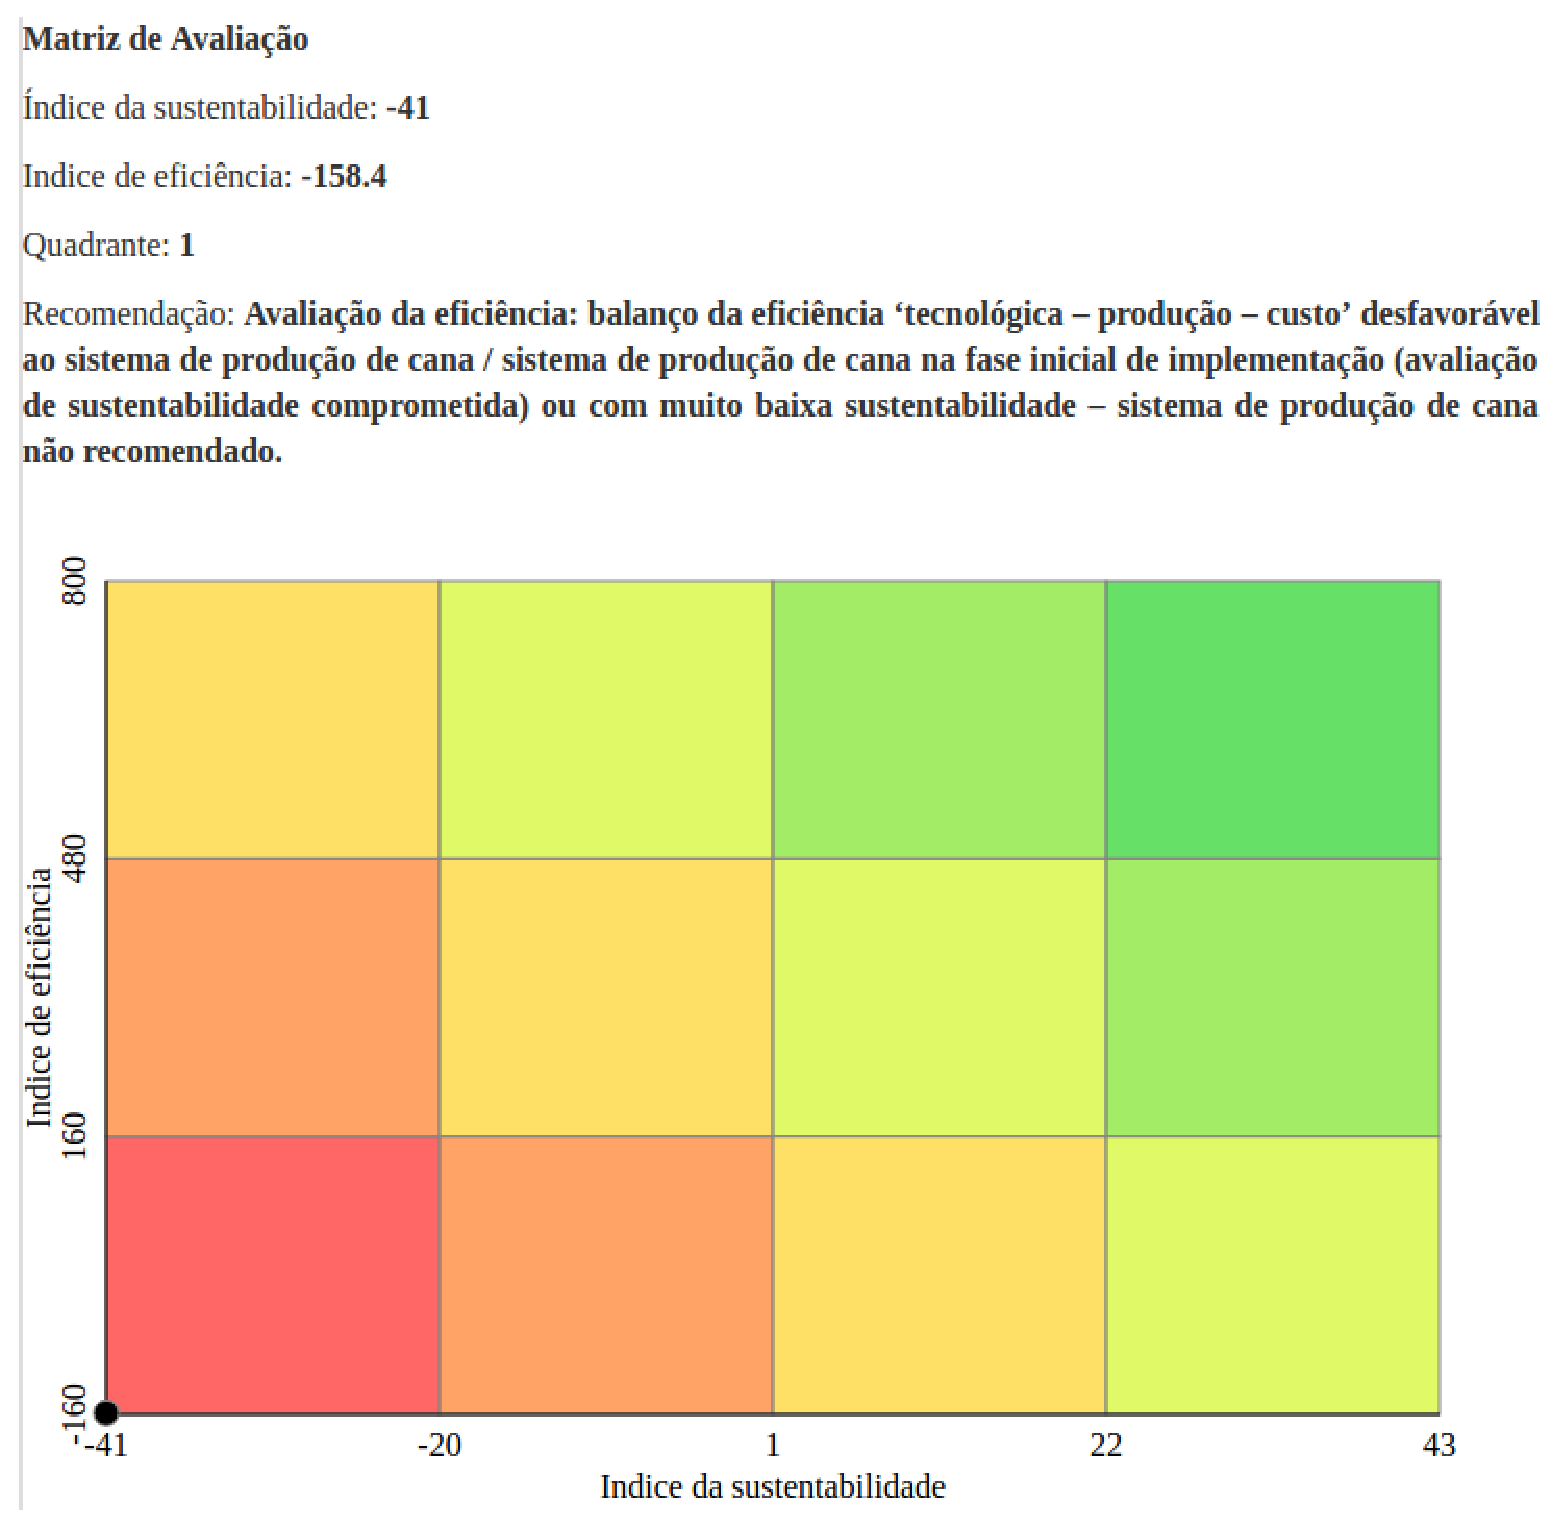
\includegraphics[width=0.8\columnwidth]{figures/Minimum}
\par\end{centering}
\caption{Matriz de Sustentabilidade com valores mínimos.\label{fig:Matriz-de-sustentabilidade-Maximos}}

\end{figure}

Um dos aspectos importantes da ferramenta, é que ela permite que os
próprios especialistas mudem, em tempo real, as fórmulas do método
de avaliação, permitindo fazer ajustes finos no método. Essa funcionalidade
permitiu descobrir e avaliar rapidamente um problema do método original:
a integração de uma operação de valor de um valor absoluto na fórmula.
A possibilidade da interação direta e fácil dos especialistas, em
tempo real, com o sistema permitiu demostrar agilmente possíveis cenários
de resolução do problema e aceitar rapidamente uma solução, proposta
pelo autor.

\section{Avaliação do SAD SustenAgro e do Framework Decisioner: }

A partir da avaliação da ontologia, da implementação do método SustenAgro
e do desenvolvimento das Web UI realizou-se uma avaliação do SAD com
a finalidade de avaliar a integração desses componentes.
\begin{description}
\item [{Data}] 18 de maio do 2016 até o dia 22 de junho do 2016
\item [{Participantes}] Usuários especialistas e usuários finais.
\item [{Local}] Instituto de Ciências Matemáticas e de Computação (ICMC-USP)
\item [{Técnica}] Teste de usabilidade
\end{description}
Para realizar uma avaliação integral do SAD SustenAgro e do Framework
Decisioner, foi necessário fazer testes de usabilidade com usuários
de ambos os perfis do sistema (especialistas de domínio e usuários
finais). Essa avaliação foi realizada com a maioria dos membros da
equipe SustenAgro e com usuários finais, de maneira remota e independente,
totalizando 8 avaliações.

A avaliação consistiu em realizar um conjunto de tarefas com o SAD
SustenAgro v1.0 e responder se foi possível terminar a tarefa e as
sugestões. As tarefas e perguntas solicitadas aos usuários estão listadas
no Apêndice \ref{sec:Formul=0000E1rio-de-avalia=0000E7=0000E3o-SustenAgro}
e permitiram gerar os seguintes resultados das avaliações:

\begin{longtable}{|>{\centering}p{0.2\columnwidth}|>{\centering}p{0.2\columnwidth}|>{\centering}p{0.6\columnwidth}|}
\hline 
\textbf{\small{}Perfil de Usuário} & \textbf{\small{}Avaliação} & \textbf{\small{}Sugestões}\tabularnewline
\hline 
\hline 
{\small{}Usuário final 1} & {\small{}Positiva, realizou as 5 tarefas de usuário final com sucesso} & \begin{itemize}
\item {\small{}Aumentar a ajuda para cada funcionalidade}{\small \par}
\item {\small{}Barra de progresso durante a avaliação}{\small \par}
\item {\small{}Resultados de avaliação mais detalhados}
\end{itemize}
\tabularnewline
\hline 
\hline 
{\small{}Usuário final 2} & {\small{}Positiva, realizou as 5 tarefas de usuário final com sucesso} & \begin{itemize}
\item {\small{}Melhorar a explicação do processo de avaliação}{\small \par}
\item {\small{}Resultados numéricos com formatação }
\end{itemize}
\tabularnewline
\hline 
\hline 
{\small{}Usuário final 3} & {\small{}Positiva, realizou as 5 tarefas de usuário final com sucesso} & \begin{itemize}
\item {\small{}Segurança no cadastro da senha}{\small \par}
\item {\small{}Melhorar a localização do botão avaliar}{\small \par}
\item {\small{}Remover }\foreignlanguage{english}{{\small{}scroll}}{\small{}
externo}{\small \par}
\item {\small{}Salvar automaticamente os dados}
\end{itemize}
\tabularnewline
\hline 
\hline 
{\small{}Especialista em sustentabilidade} & {\small{}Positiva, realizou as 5 tarefas de usuário e as 5 tarefas
de especialista de domínio com sucesso} & \begin{itemize}
\item {\small{}Definir e acrescentar os termos de uso}{\small \par}
\item {\small{}Melhorar a sequencia de telas durante o cadastro de novo
usuário}{\small \par}
\item {\small{}Balão explicativo dos campos do formulário de nova unidade
produtiva, especificamente a propriedade de publicação dos dados}{\small \par}
\item {\small{}Definir o limite de caráteres para o campo de justificativa}{\small \par}
\item {\small{}Salvar avaliação ao mudar de aba}{\small \par}
\item {\small{}Justificativas sempre visíveis na tela de resultados.}{\small \par}
\item {\small{}Acrescentar bandeira em inglês e termos de uso}
\end{itemize}
\tabularnewline
\hline 
\hline 
{\small{}Especialista economia} & {\small{}Positiva, realizou as 5 tarefas de usuário e as 5 tarefas
de especialista de domínio com sucesso} & \begin{itemize}
\item {\small{}Salvar dados da seção automaticamente}{\small \par}
\item {\small{}Mudanças em alguns }\foreignlanguage{english}{{\small{}labels}}{\small \par}
\item {\small{}Mudanças nos indicadores}{\small \par}
\item {\small{}Componentes gráficos para representar os dados }{\small \par}
\item {\small{}Editor visual de ontologia e internacionalização}
\end{itemize}
\tabularnewline
\hline 
\hline 
{\small{}Especialista em ontologias} & {\small{}Positiva, realizou as 5 tarefas de usuário final com sucesso} & \begin{itemize}
\item {\small{}Melhorar a apresentação do botão salvar}{\small \par}
\item {\small{}Indicadores em forma de pergunta com verbo e simbolo de pergunta}{\small \par}
\item {\small{}Informar a possibilidade de edição de indicadores }
\end{itemize}
\tabularnewline
\hline 
\hline 
{\small{}Especialista agricultura} & {\small{}Positiva, realizou as 5 tarefas de usuário final com sucesso} & \begin{itemize}
\item {\small{}Cadastrar mais de uma microrregião}{\small \par}
\item {\small{}Remover }\foreignlanguage{english}{{\small{}scroll}}{\small{}
externo, mudanças em vários indicadores}{\small \par}
\item {\small{}Melhorar a localização do botão salvar e avaliar}{\small \par}
\item {\small{}Salvar a seção para não perder os dados}{\small \par}
\item {\small{}Melhorar a apresentação do pdf}
\end{itemize}
\tabularnewline
\hline 
\hline 
{\small{}Especialista em computação} & {\small{}Positiva, realizou as 5 tarefas de usuário final com sucesso} & \begin{itemize}
\item {\small{}Salvar a seção e os dados dela em tempo real}{\small \par}
\item {\small{}Integrar sistemas externos para poupar informação (caracterização
da unidade produtiva) }
\end{itemize}
\tabularnewline
\hline 
\end{longtable}

\begin{table}[H]
\caption{Avaliação do SAD SustenAgro}
\end{table}

A partir dessa avaliação integral, feita por usuários finais e administradores,
foram definidas várias melhorias a serem realizadas no Framework Decisioner
e o SAD SustenAgro. Devido às limitações de tempo e de desenvolvedores,
foram implementados apenas os ajustes visuais nas web UI, melhoras
na apresentação dos resultados, na geração do PDF e, principalmente,
a inclusão da linguagem inglês. Essa última mudança foi selecionada
como de especial importância, por parte dos especialistas. Neste documento,
são apresentadas várias telas, tanto em português como em inglês,
que foram geradas a partir da implementação dessa funcionalidade.
\selectlanguage{english}%

\section{Workshop\foreignlanguage{brazil}{: validação do software SustenAgro
v1.0 com equipe de especialistas.}}

\selectlanguage{brazil}%
A partir das melhoras realizadas na avaliação interna pelos dois tipos
de usuários do SAD SustenAgro, o sistema foi disponibilizado em servidos
web do ICMC. Esta publicação permitiu dar suporte a uma avaliação
no formato de \foreignlanguage{english}{workshop} com especialistas
de diversos perfis que tinham interesse no SAD SustenAgro. O \foreignlanguage{english}{Workshop}
foi intitulado ``Validação do software SustenAgro'', os detalhes
do \foreignlanguage{english}{workshop} são apresentados a seguir.
\begin{description}
\item [{Data}] 14 de julho do 2016
\item [{Participantes}] Equipe do projeto SustenAgro de várias unidades
da Embrapa
\item [{Local}] Embrapa Informática Agropecuária - Campinas
\item [{Técnica}] Delphi
\end{description}
O \foreignlanguage{english}{workshop} teve o objetivo de avaliar a
qualidade e acuidade do SAD SustenAgro em termos da clareza da informação
técnica apresentada nas interfaces, com vistas a garantir o entendimento
do usuário e possibilitar que a avaliação da sustentabilidade do sistema
de produção de cana-de-açúcar seja realizada da melhor forma possível. 

No \foreignlanguage{english}{workshop} foi apresentado o formulário
de avaliação (Seção \ref{sec:Formulario-Delphi-Workshop}) usando
a técnica \foreignlanguage{english}{Delphi} \citep{wright1985tecnica},
a um grupo de especialistas com perfis de varias áreas do conhecimento,
entre eles destacam-se:
\begin{itemize}
\item Especialista em sustentabilidade
\item Especialista em ciências agrícolas
\item Especialista em modelagem de conhecimento
\item Especialista em ciência e Tecnologia do Bioetanol
\item Especialista em ciências da computação
\item Especialista em economia agrícola
\item Especialista em biotecnologia
\item Mestrando em ciências da computação (sistemas web e multimídia)
\item Mestrando em Planejamento de Sistemas Energéticos
\end{itemize}
As interações com o sistema foram filmadas enquanto os usuários executavam
uma lista de tarefas. Monitores do ICMC ficavam estimulando os usuários
a falar o que estavam pensando (técnica Think Aloud ) e os questionavam,
quando tinham alguma dificuldade de interação. Ao final, houve um
\foreignlanguage{english}{debriefing} e foram também colhidas mais
sugestões de mudança. 

Os especialistas aprovaram a ferramenta tanto na interação como no
conteúdo dela, com as seguintes sugestões:
\begin{itemize}
\item As perguntas dos indicadores não são de fácil interpretação.
\item Colocar mais informações na interface para facilitar o uso dela, por
exemplo o significado de alinhamento dos indicadores.
\item Alguns indicadores estão repetidos.
\item Os resultados da avaliação deveriam estar por dimensão.
\item Demora para salvar os dados inseridos.
\item A informação dos site tem inconsistências em relação à informação
do pdf gerado.
\item A recomendações do relatório precisam mais detalhamento.
\end{itemize}
É interessante que muitas das sugestões não tem haver com aspectos
computacionais ou de interface, mas sim com o processo de avaliação
de sustentabilidade. Esse processo é de inteira responsabilidade dos
especialistas de domínio (e foge totalmente do escopo deste trabalho).
Isso foi um ponto positivo. É natural que especialistas em sustentabilidade
estejam muito mais interessados na sua área do que nos aspectos computacionais
do SAD SustenAgro. Uma boa interface é aquela que desaparece da mente
do usuário e permite que este se foque na sua tarefa. Neste caso,
a avaliação de sustentabilidade. Acreditamos que o SAD SustenAgro
atendeu bem a esse requisito.

\section{Avaliação de SAD SustenAgro nos servidores da Embrapa}

A partir da aprovação do SAD SustenAgro, por parte dos especialistas
no \foreignlanguage{english}{workshop}, foi autorizada a instalação
da ferramenta nos servidores da Embrapa Meio Ambiente. Essa instalação
foi um esforço coordenado entre o desenvolvedor do framework Decisioner
(o autor deste trabalho) e técnicos de informática da Embrapa.
\begin{description}
\item [{Data}] 18 de agosto do 2016
\item [{Participantes}] Especialista em Sustentabilidade e especialista
em TI
\item [{Local}] Embrapa Meio Ambiente - Campinas
\item [{Técnica}] Teste de usabilidade
\end{description}
A instalação, coordenada pelo desenvolvedor do Framework Decisioner
e técnicos da Embrapa, foi problemática. A Embrapa não autoriza o
acesso físico ou via ssh aos servidor por parte de profissionais externos.
Por esta razão, foi criado um documento de instalação, descrito no
Apêndice \ref{chap:Instalation}. Nele estão as instruções para instalar
o Framework Decisioner e instanciar o SAD SustenAgro.

A instalação foi exitosa e o sistema está funcionando no endereço
\url{https://sustenagro.embrapa.br/}. Atualmente o endereço não está
no ar, pois o SAD SustenAgro está em processo de registro no Instituto
Nacional de Propriedade Intelectual (INPI), em nome da Embrapa e USP,
e a Embrapa ter uma política de exigir esse registro para liberação
para uso externo.

\section{Conclusões}

Essas avaliações permitiram verificar que os requisitos do Framework
Decisioner e do SAD SustenAgro foram implementados corretamente e
que atenderam as necessidades dos especialistas de domínio e usuários
finais, identificadas nos levantamentos de requisitos.

As avaliações ocorreram em diferentes fases do projeto e cada uma
trouxe correções e melhoras que foram implementadas, na medida do
possível, segundo a relevância de cada mudança e o tempo disponível
para desenvolvedor do projeto. Por ter sido desenvolvido em um processo
cíclico, cada iteração acrescentou novas funcionalidades que fizeram
mudar a arquitetura dos sistemas, gerando \foreignlanguage{english}{bugs}
e inconsistências. Na versão 1.0, os sistemas contam com funcionalidades
estáveis que permitem fornecer os serviços implementados. Correções
e sugestões recebidas durante a avaliação e não implementadas por
problema de tempo, foram deixadas como trabalhos futuros, que serão
apresentados no próximo capítulo juntamente com as conclusões.


\chapter{Conclusão}

Os resultados obtidos são: 
\begin{enumerate}
\item Ontologia em formatos da web semântica (RDF/OWL) da avaliação da sustentabilidade
no sistema de cana-de-açúcar. 
\item Protótipo de ontologia de interfaces gráficas em formatos da web semântica
(RDF/OWL) 
\item Linguagem de domínio especifico DSL, Decisioner, para definir e permitir
administrar os parâmetros e processos do sistema SustenAgro 
\item Protótipo de sistema de geração de interfaces suportado nas tecnologias
da web semântica 
\item Formulários para recolha de dados sobre sustentabilidade em cana-de-açúcar,
e o processo de colheita dos dados de algumas usinas do estado de
São Paulo 
\item Protótipo do sistema web Sustenagro que integra as ontologias e a
DSL, fornecendo um comportamento configurável em tempo de execução
dos parâmetros, processos e das interfaces gráficas de usuário
\end{enumerate}
Uma das finalidades deste projeto é construir um gerador de sistemas
de apoio a decisão que consiga suportar outros domínios de conhecimento,
propondo para a comunidade uma metodologia de desenvolvimento e manutenção
que fique simples para os usuários finais e assim permitir que os
especialistas no domínio façam as mudanças sem precisas dos especialistas
de T.I.

\section{Trabalhos Futuros}

Este capítulo apresenta os resultados estão uma versão da ontologia
de domínio do SustenAgro e artefatos para o desenvolvimento da interface
visual do sistema: User Stories, Scenarios, Story Boards, Mockups
e um protótipo para a interface do SustenAgro.

Os resultados obtidos são: 
\begin{enumerate}
\item Ontologia em formatos da web semântica (RDF/OWL) da avaliação da sustentabilidade
no sistema de cana-de-açúcar. 
\item Protótipo de ontologia de interfaces gráficas em formatos da web semântica
(RDF/OWL) 
\item Linguagem de domínio especifico DSL, Decisioner, para definir e permitir
administrar os parâmetros e processos do sistema SustenAgro 
\item Protótipo de sistema de geração de interfaces suportado nas tecnologias
da web semântica 
\item Formulários para recolha de dados sobre sustentabilidade em cana-de-açúcar,
e o processo de colheita dos dados de algumas usinas do estado de
São Paulo 
\item Protótipo do sistema web Sustenagro que integra as ontologias e a
DSL, fornecendo um comportamento configurável em tempo de execução
dos parâmetros, processos e das interfaces gráficas de usuário
\end{enumerate}
Uma das finalidades deste projeto é construir um gerador de sistemas
de apoio a decisão que consiga suportar outros domínios de conhecimento,
propondo para a comunidade uma metodologia de desenvolvimento e manutenção
que fique simples para os usuários finais e assim permitir que os
especialistas no domínio façam as mudanças sem precisas dos especialistas
de T.I.


\bibliographystyle{abntex2-alf}
\bibliography{references/references}

\end{document}
